


\section{Esercizio 6.3.1}

\subsection{Problem Statement}
Scrivere un programma che risolva un'equazione differenziale utilizzando il metodo RK2.
\noindent Testare il programma con l'equazione differenziale dell'oscillatore armonico con i seguenti valori iniziali:

\[
\ddot{\theta}(t) = -\theta, \quad \text{con } \theta(0) = 0 \text{ e } \dot{\theta}(0) = 1,
\]

\begin{itemize}
    \item Ottenere la soluzione analitica $\theta(t)$ e confrontarla con la soluzione numerica $\eta(t; h)$ ottenuta tramite i metodi RK2 ed Eulero.
    \item Tracciare i grafici di $\theta(t)$, $\dot{\theta}(t)$ e il diagramma dello spazio delle fasi $\dot{\theta}(\theta)$.
    \item Studiare l'errore $\mathcal{E}(t, h) = \eta(t, h) - \theta(t)$ in funzione del passo $h$ a un tempo $t$ fissato e dimostrare che i metodi hanno l'ordine di precisione atteso.
\end{itemize}


\subsection{Premessa Teorica}
In questa sezione decidiamo di analizzare alcuni problemi di risoluzione di \textit{ODE}. In generale definiamo:
\[
\frac{d y}{dx} = f(x, y(x)), \quad y(x_0) = y_0,
\]

come il problema al valore iniziale, del primo ordine. L'obiettivo è quindi determinare la funzione $y(x)$, conoscendo una condizione sulla derivata prima ($f$) e il valore della funzione in un punto $(y_0)$.

\subsection{Metodi Numerici e Algoritmi}
Si può definire un primo metodo approssimativo, che è quello di Eulero: dalla semplice riscrittura della parte sinistra dell'equazione usando le differenze finite, possiamo avere una prima via di risoluzione, con un algoritmo iterativo.\\
In particolare il "Forward Euler Method"
\footnote{
Così denominato poiché fa uso della definizione \textit{forward} della differenza finita. Sarà quindi possibile definire anche un algoritmo \textit{backward}, ma con caratteristiche leggermente diverse e che non approfondiamo in questa sezione.
}
:
\[
    \eta(x+h, h) = \eta(x,h) + h f(x, \eta(x,h))
\]

dove abbiamo denominato $\eta(x+h, h)$ la soluzione numerica di della soluzione all'istante $x+h$: questa sarà in generale differente dalla soluzione vera $y(x)$.\\
Mantenendo la stessa notazione, ma passando ad un nuovo approccio, posso definire il metodo di Runge-Kutta di ordine 2 come:
\[
\eta(x+ h,h) = \eta(x,h) + h f\left(x + \frac{1}{2}h, \eta(x,h) + \frac{1}{2}hf(x, \eta(x,h))\right)
\]

L'interpretazione di quello che fa numericamente il metodo è da ritrovare nella sua solita denominazione di \textit{midpoint method}: per stimare il valore della funzione in $x+h$, conoscendo il suo valore in $x$, possiamo usare la pendenza in $x$. Approssimare la funzione ad una retta è una possibile approssimazione per uno step piccolo; la scelta di RK2 è di fare due valutazioni della funzione, una volta per stimare il valore nel punto intermedio, cioè a $x+h/2$, la seconda per fornire una stima più accurata della derivata al passo, che viene poi utilizzata nell’aggiornamento finale. Questo approccio è quello che differenzia Eulero e RK2, e che permette al secondo di migliorare notevolmente la sua accuratezza e stabilità.\\
Per entrambi i casi gli algoritmi sono iterativi: ad un passo n-esimo la soluzione numerica $\eta(x+ n h,h)$ è un'approssimazione di quella esatta $y(x + n h)$.

\medskip\noindent
Si può dimostrare che per il metodo di Eulero l'errore locale, cioè per la singola iterazione, con passo $h$, scala in modo quadratico. Per l'algoritmo RK2 vale la convergenza cubica.\\
In generale l'errore globale, che tiene conto dell'accumulazione degli errori ai passi n-esimi, è diverso da quello locale, solitamente maggiore: accade infatti che per questi due metodi la convergenza perda un ordine nello \textit{scaling}, perciò:
\begin{itemize}
    \item \textbf{Eulero}: scaling lineare.
    \item \textbf{RK2}: scaling quadratico.
\end{itemize}


\subsection{Risultati e Discussione}

L'oscillatore armonico è definito dall'equazione differenziale:
\[
\ddot\theta(t) +\omega^2 \theta(t) = 0
\]
La cui soluzione generale è:
\[
\theta(t) = A\cos(\omega t) + B\sin(\omega t)
\]

\noindent Nel nostro esercizio $\omega^2=1$, scegliamo $\omega=1$, e le condizioni al contorno determinano univocamente i parametri $A, B$:
\begin{align*}
    \begin{cases}
        \theta(0) = 0\\
        \dot \theta(0) = 1\\
    \end{cases}
    \quad \to \quad 
    A = 0, B= 1
\end{align*}

\[
\implies \theta(t) = \sin(t)
\]

L'idea è ora quella di confrontare il risultato analitico con quello numerico. In Fig. \ref{fig: rk2 th, dth} e \ref{fig: rk2 fasi} vediamo alcuni plot che riguardano il metodo RK2, diagrammi che mostrano il peso della scelta del passo nell'accuratezza della soluzione.\\
In Fig. \ref{fig: confr th,dth} e \ref{fig: confr fasi} i confronti sono fatti tra i due algoritmi di RK2 e Eulero, fissando un passo a $h=0.3$. 

\begin{figure}[H]
    \centering
    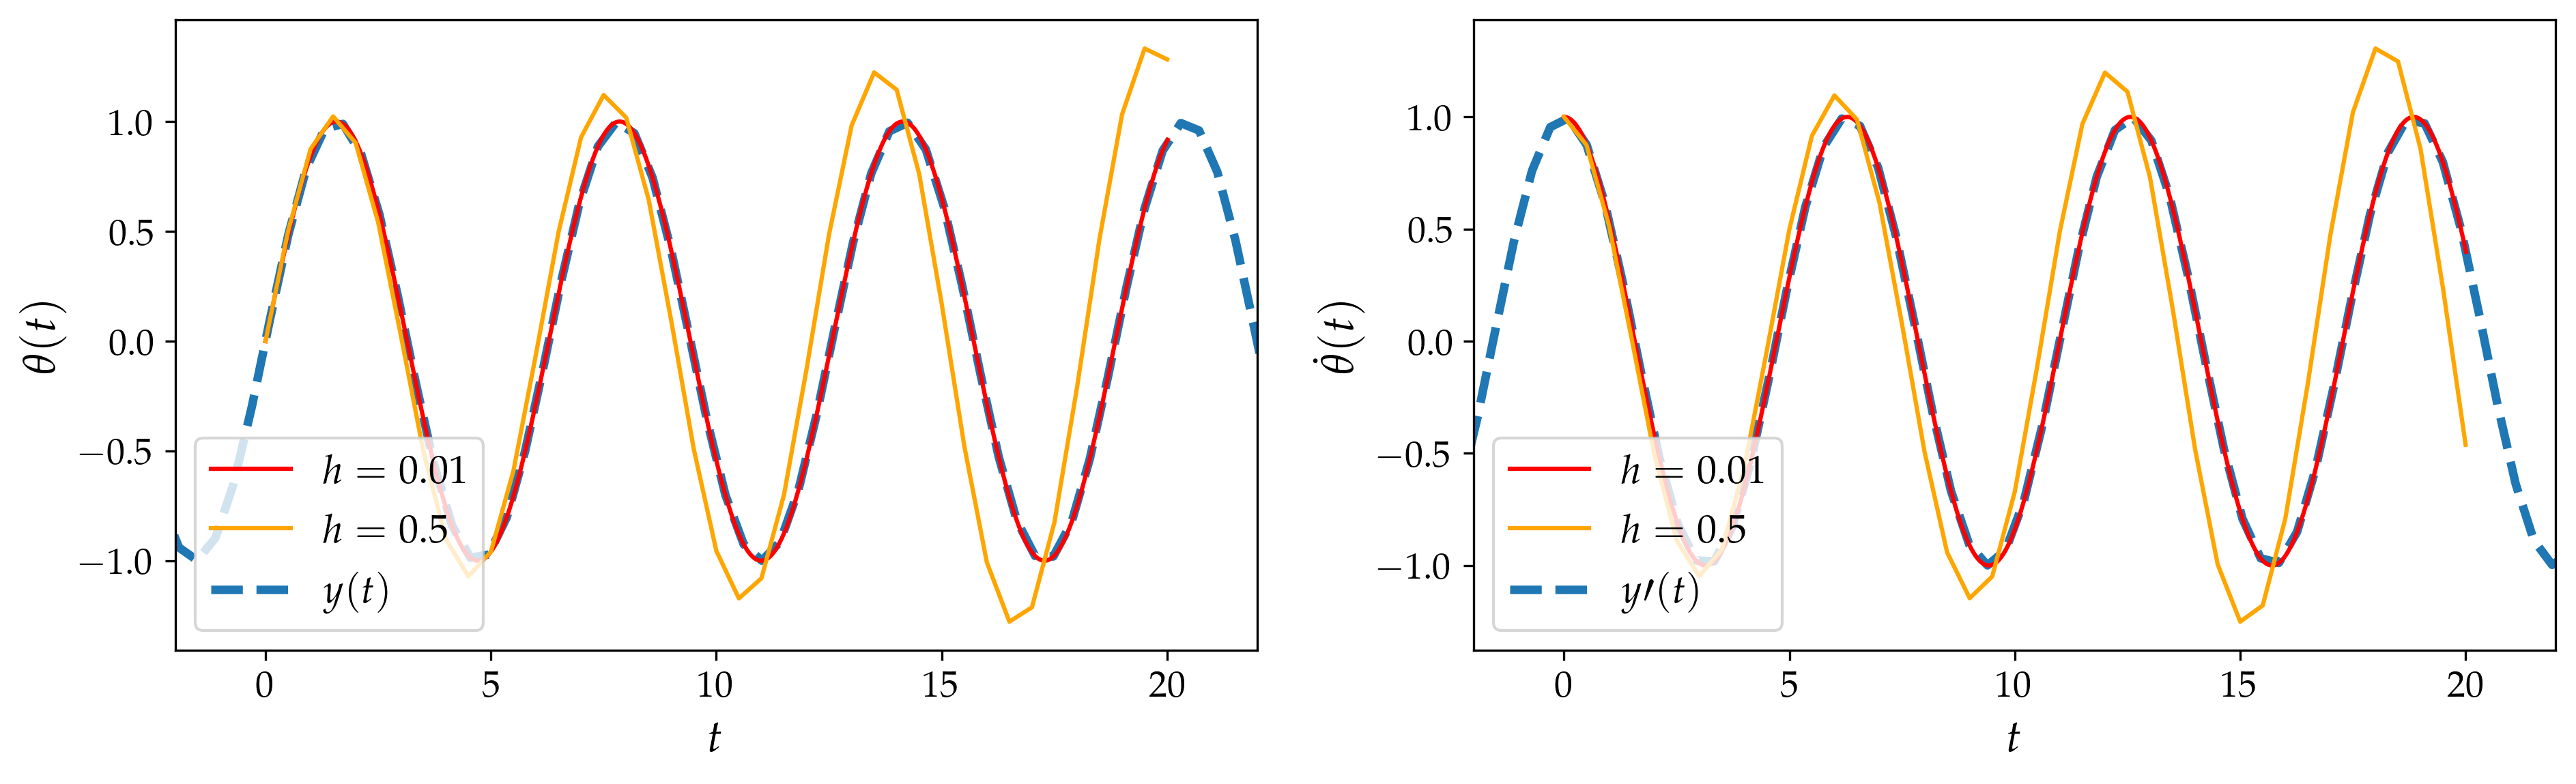
\includegraphics[width=\linewidth]{images/17/RK2_th_dth.png}
    \caption{In figura il plot che evidenzia come varia l'accuratezza del metodo RK2 con il passo, più grande o più piccolo. Come ci si aspetta, più piccolo il passo, migliore l'approssimazione di  $\eta(x+ n h,h)$ a $y(x + n h)$.}
    \label{fig: rk2 th, dth}
\end{figure}

\begin{figure}[H]
    \centering
    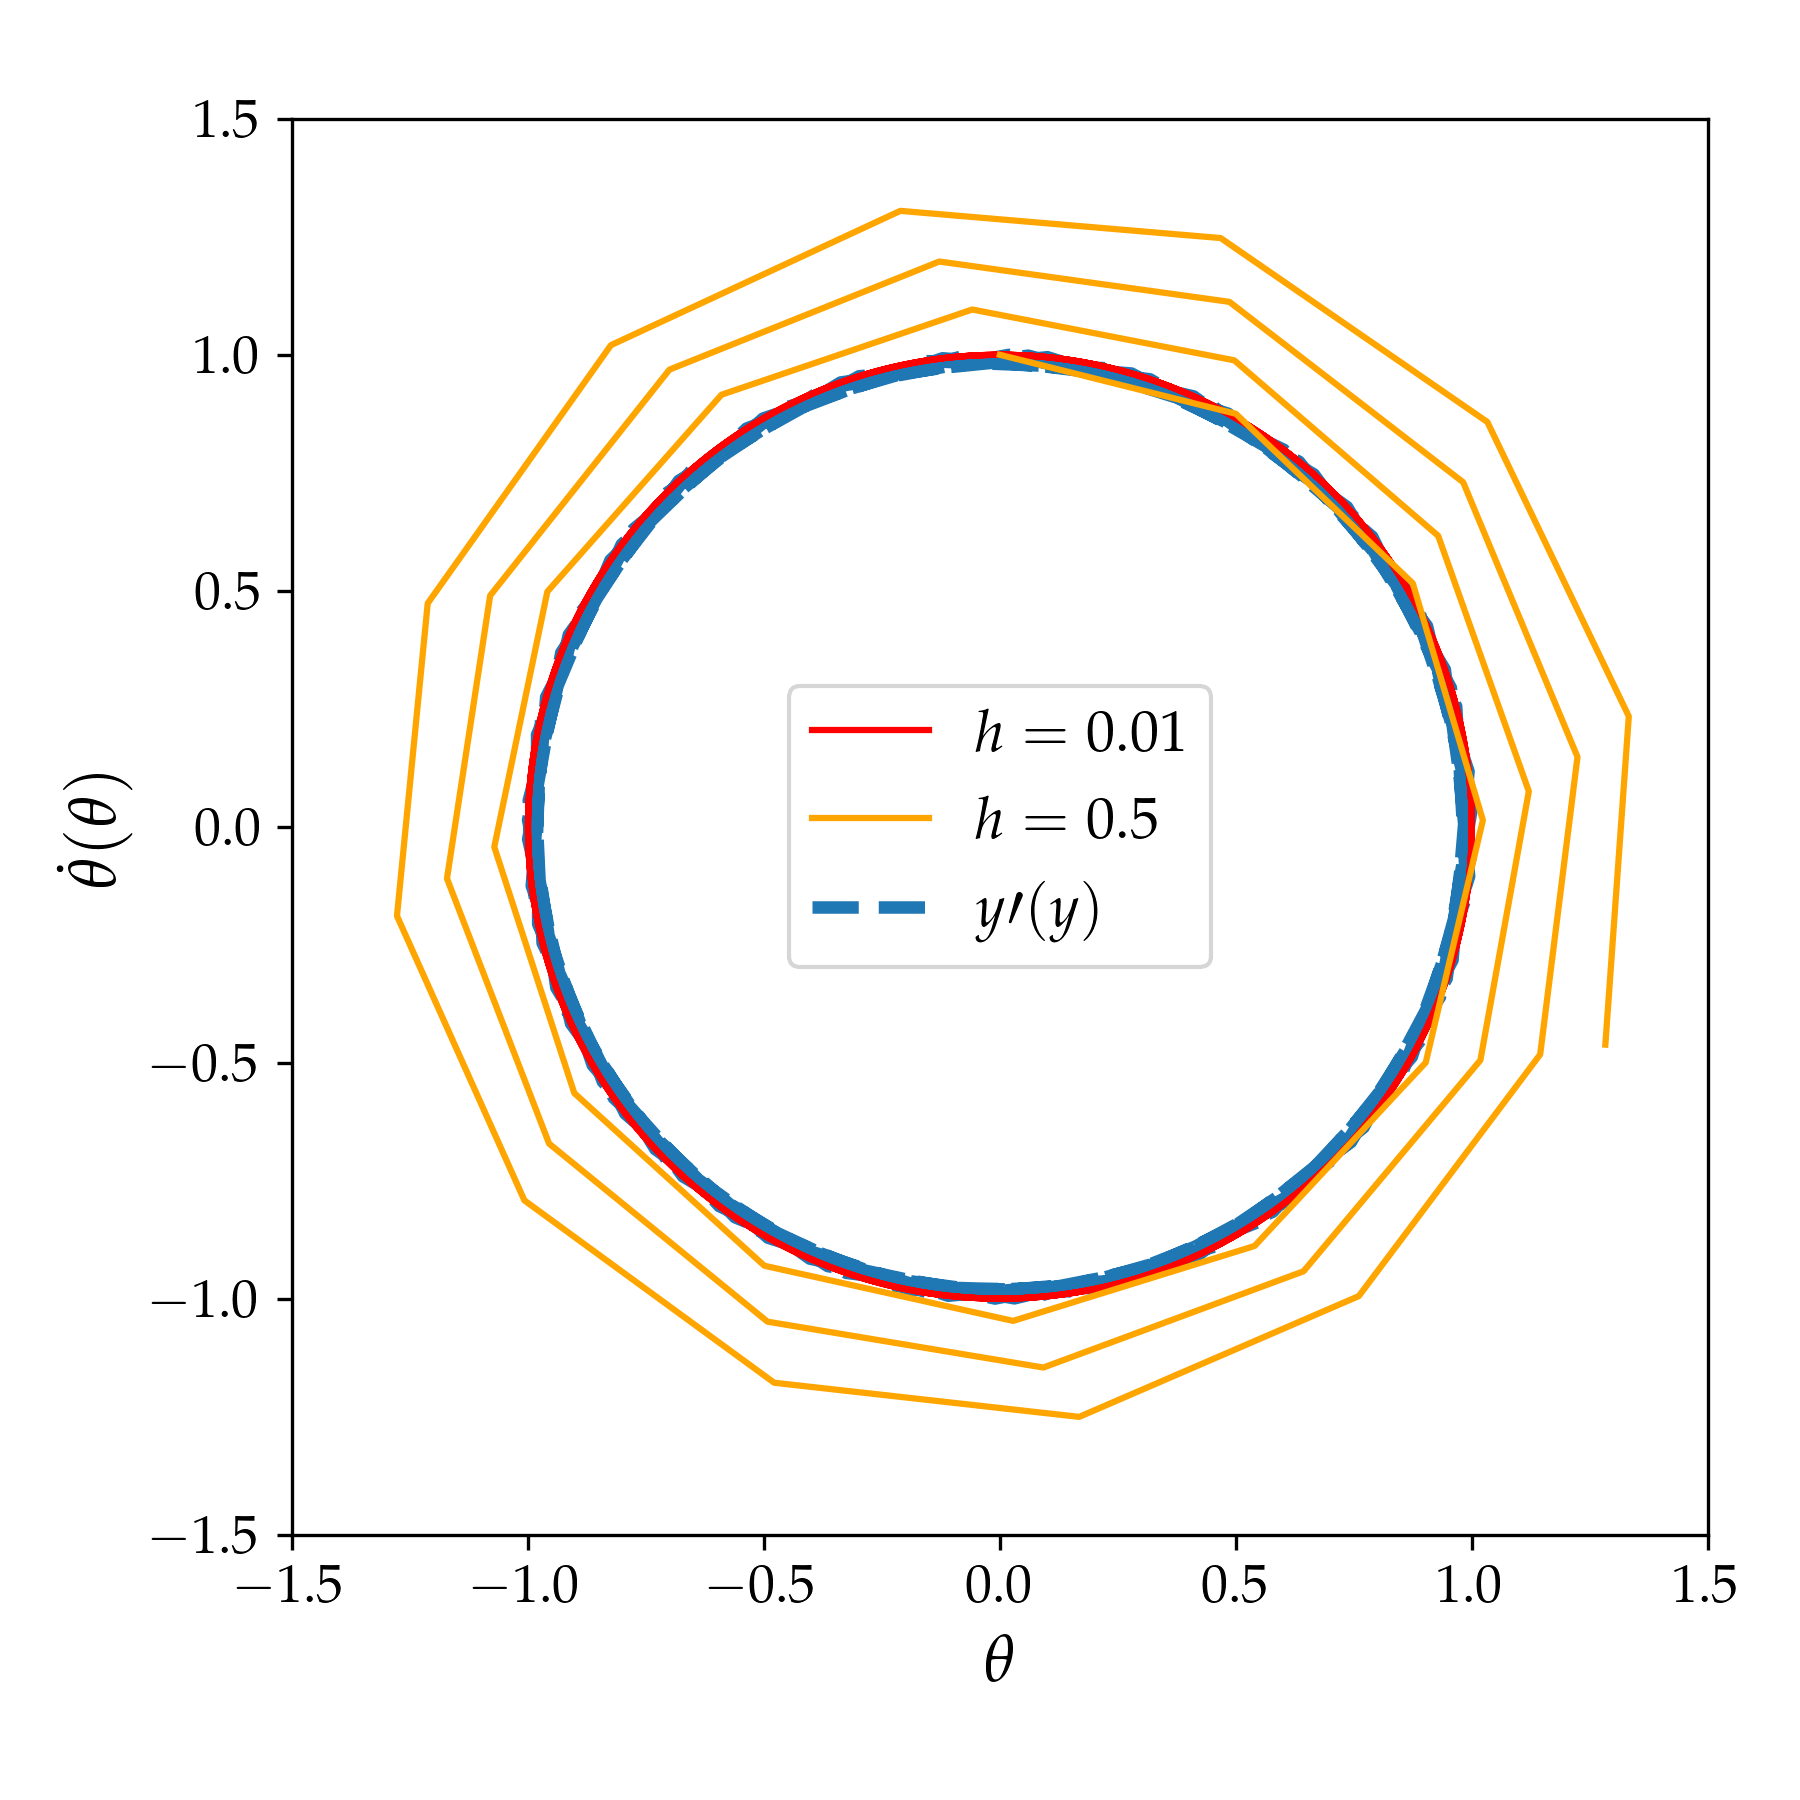
\includegraphics[width=0.6\linewidth]{images/17/RK2_fasi.png}
    \caption{Il diagramma delle fasi per RK2: si osserva un progressivo allontanamento dalla traiettoria esatta dovuto agli errori numerici accumulati, con passo di $h=0.5$, mentre l'approssimazione di $h=0.01$ è ottima nel confronto con la soluzione esatta.}
    \label{fig: rk2 fasi}
\end{figure}

\begin{figure}[H]
    \centering
    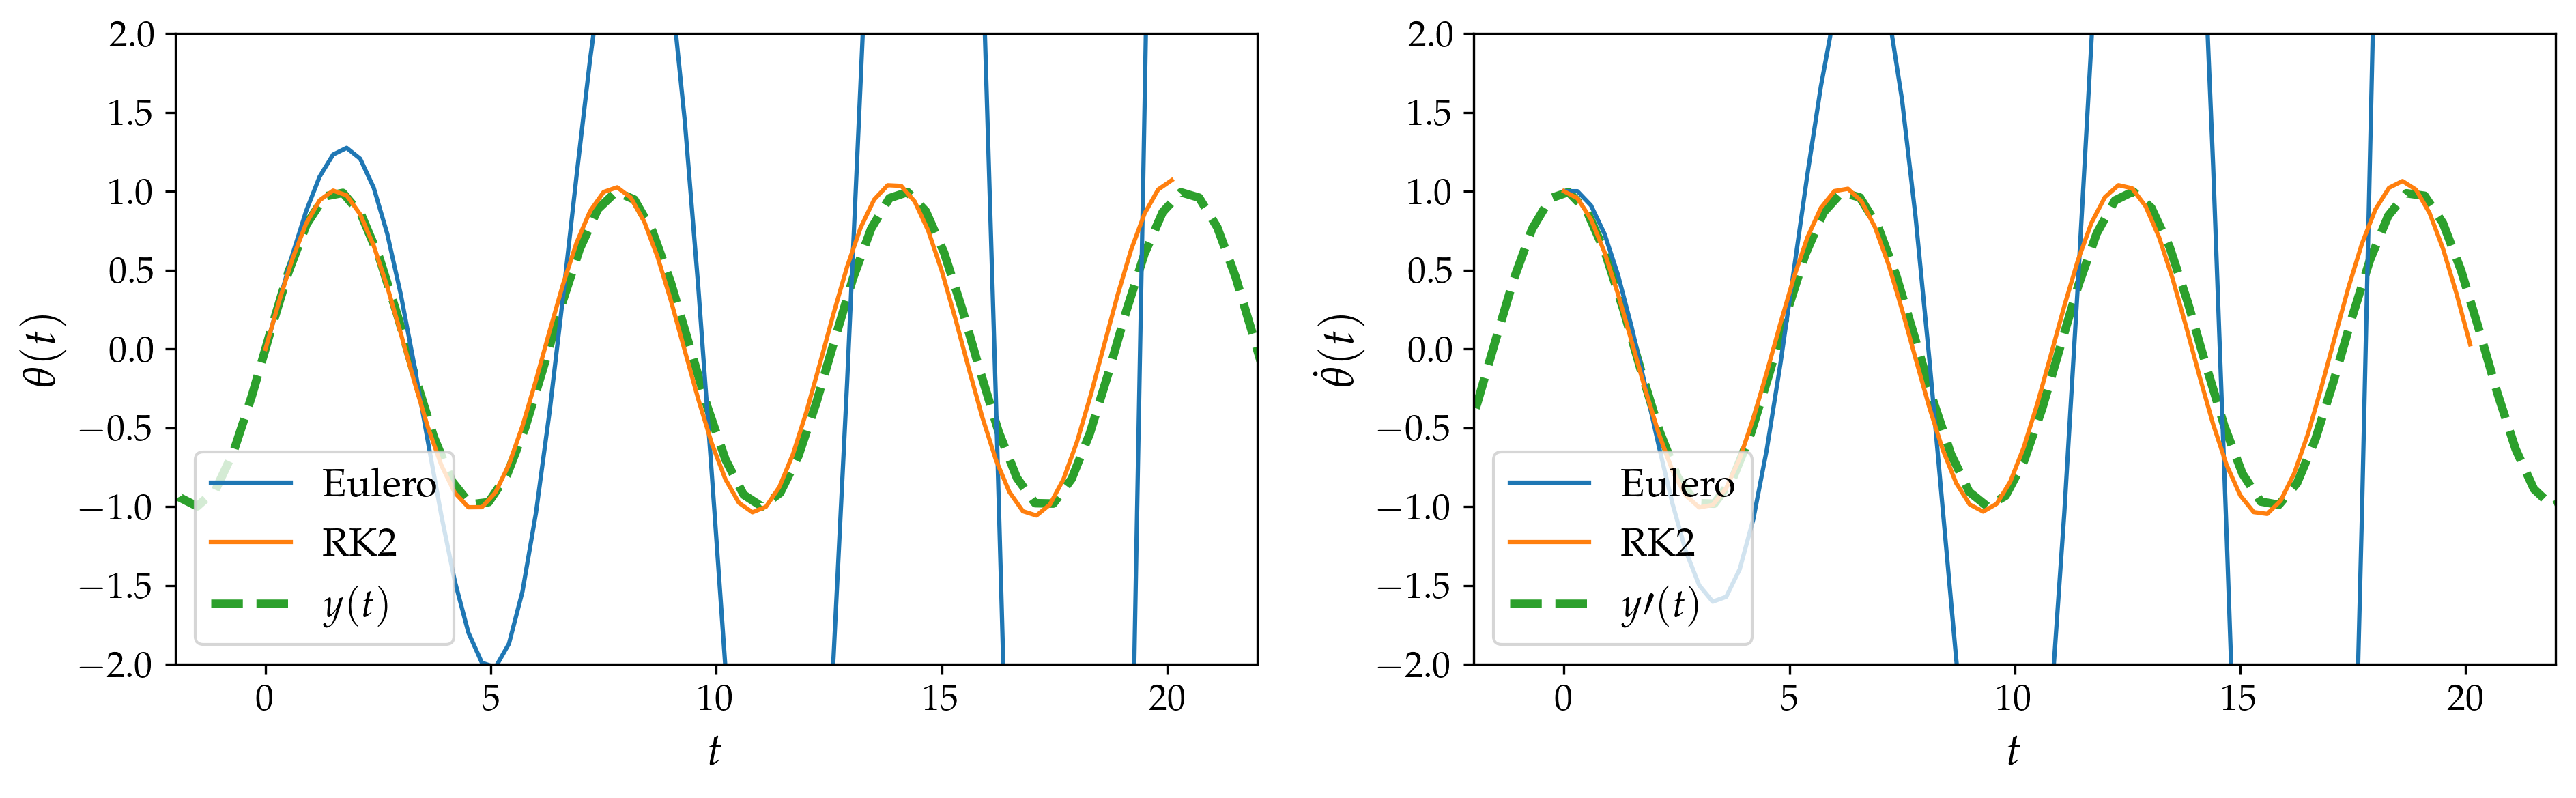
\includegraphics[width=\linewidth]{images/17/confr_th_dth.png}
    \caption{Le approssimazioni dei due metodi alla soluzione esatta: in entrambi è possibile apprezzare la maggiore stabilità della soluzione numerica di RK2, rispetto a quella di Eulero, che diverge velocemente.}
    \label{fig: confr th,dth}
\end{figure}


\begin{figure}[H]
    \centering
    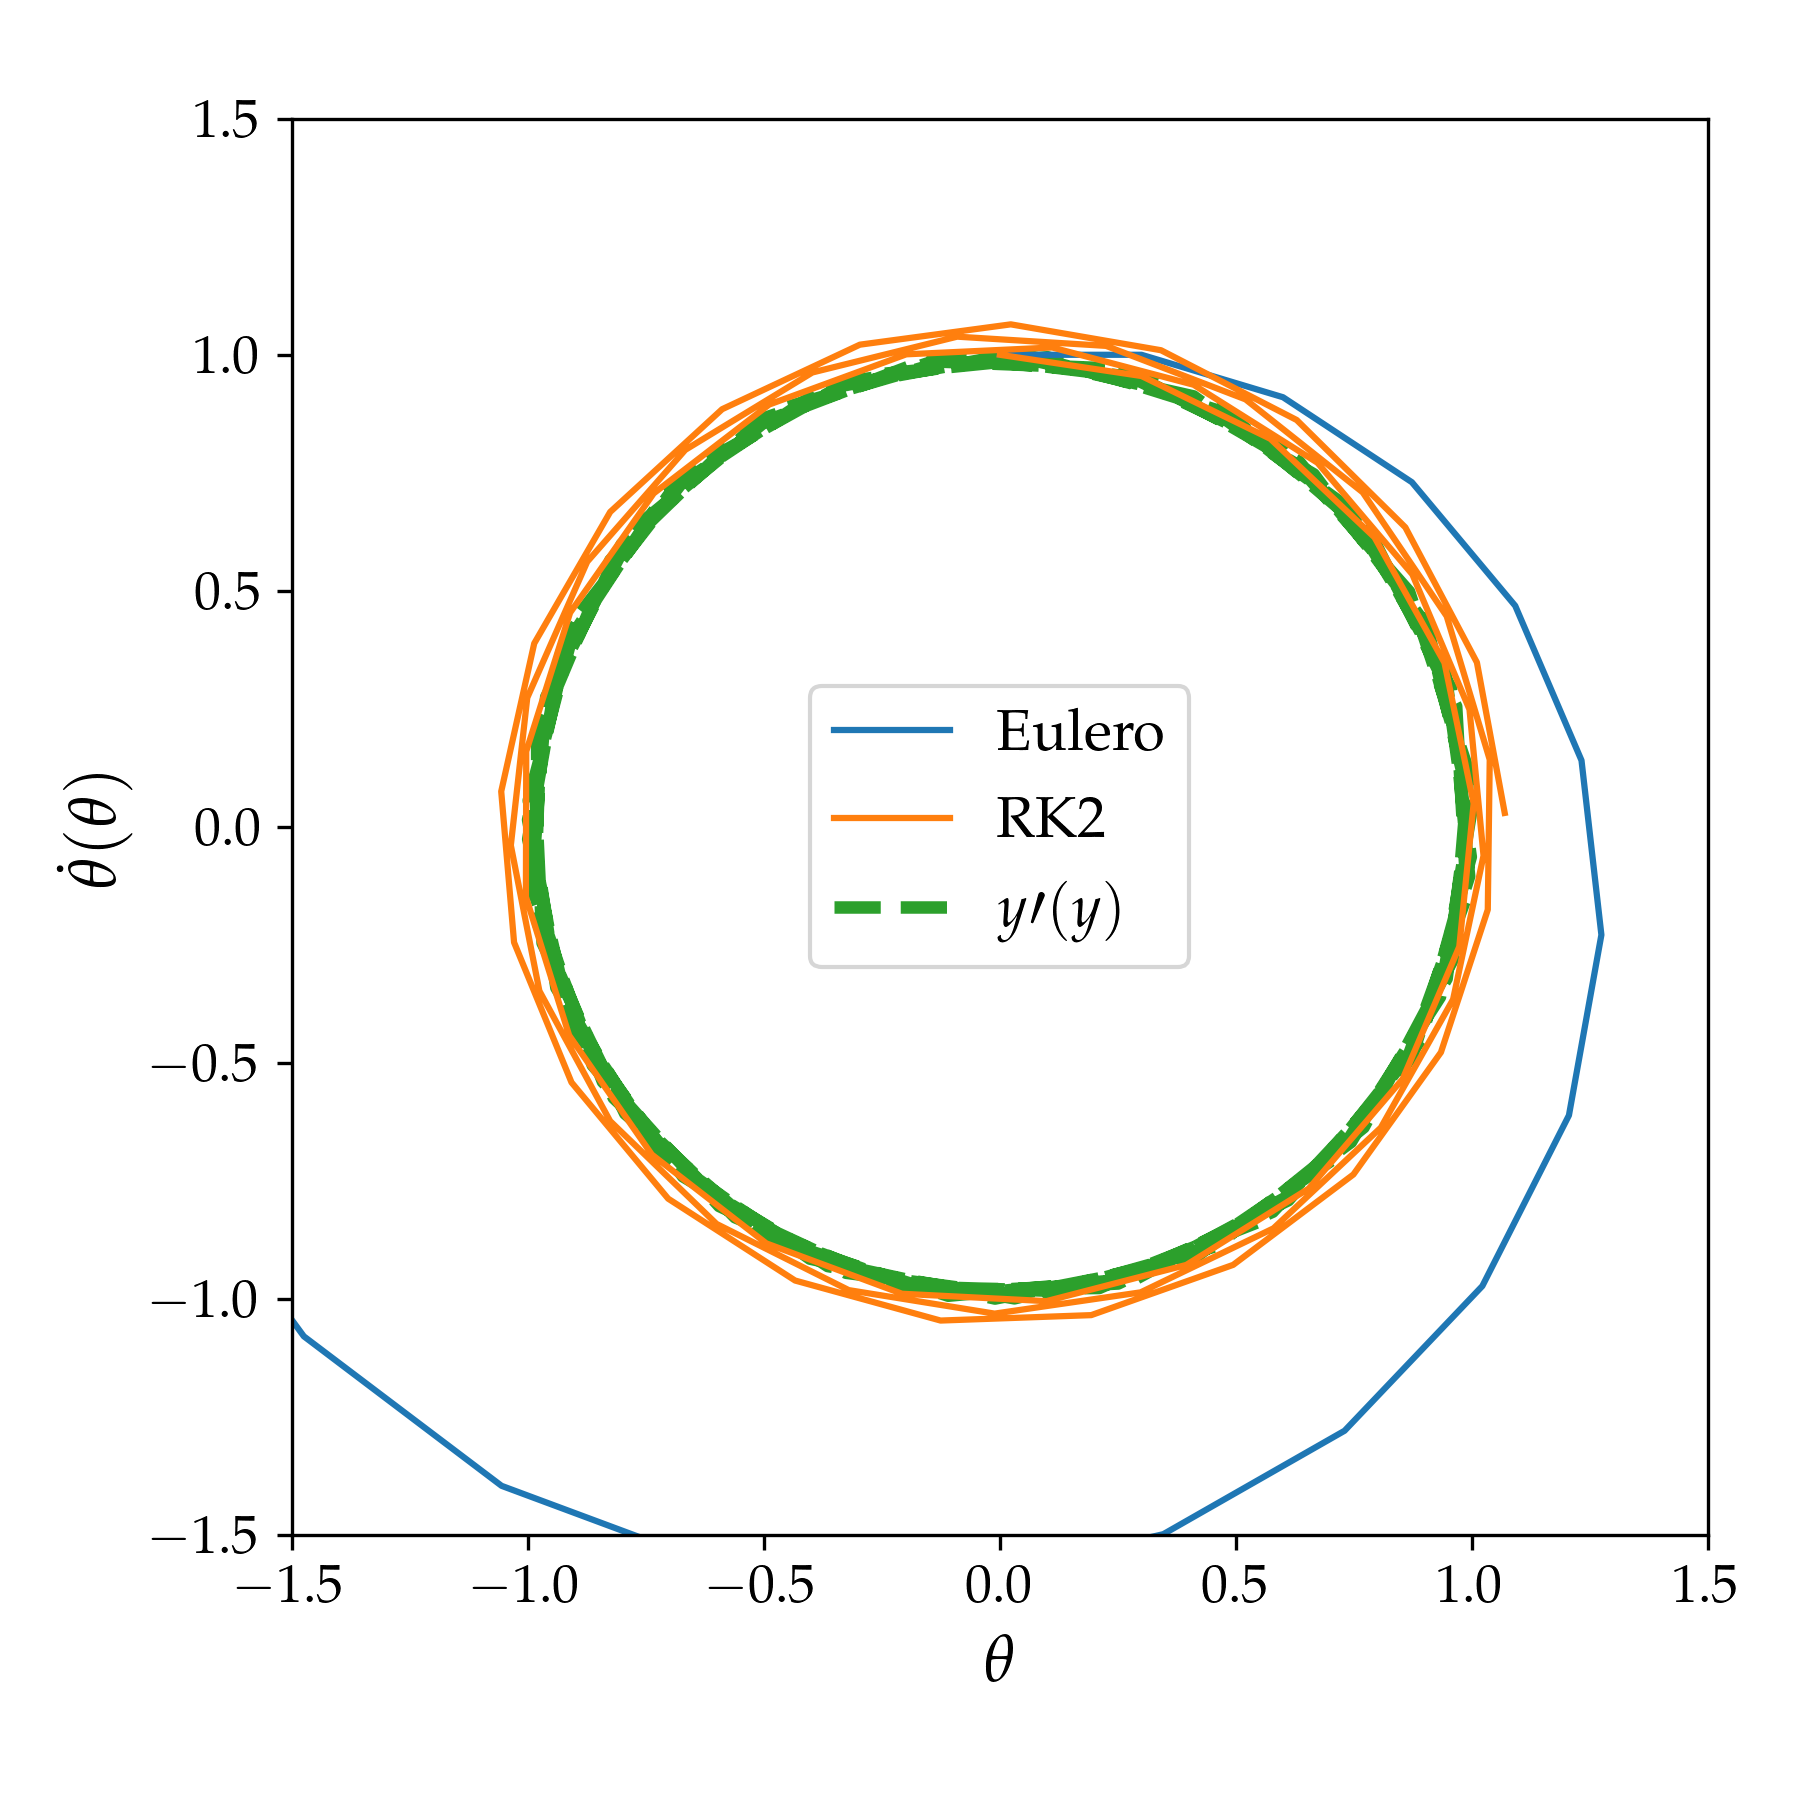
\includegraphics[width=0.6\linewidth]{images/17/confr_fasi.png}
    \caption{Il confronto tra i metodi viene esteso anche al diagramma delle fasi.}
    \label{fig: confr fasi}
\end{figure}

\noindent Lo studio dell'errore in funzione del passo $h$, ad un tempo fissato $t$ è in Fig. \ref{fig: Scaling confr}: definisco 
\[
\mathcal E(t, h) = \eta(t, h) - \theta(t)
\]
in particolare fissiamo il tempo $t=1$ e procediamo con l'analisi della convergenza dei metodi.

\begin{figure}[H]
    \centering
    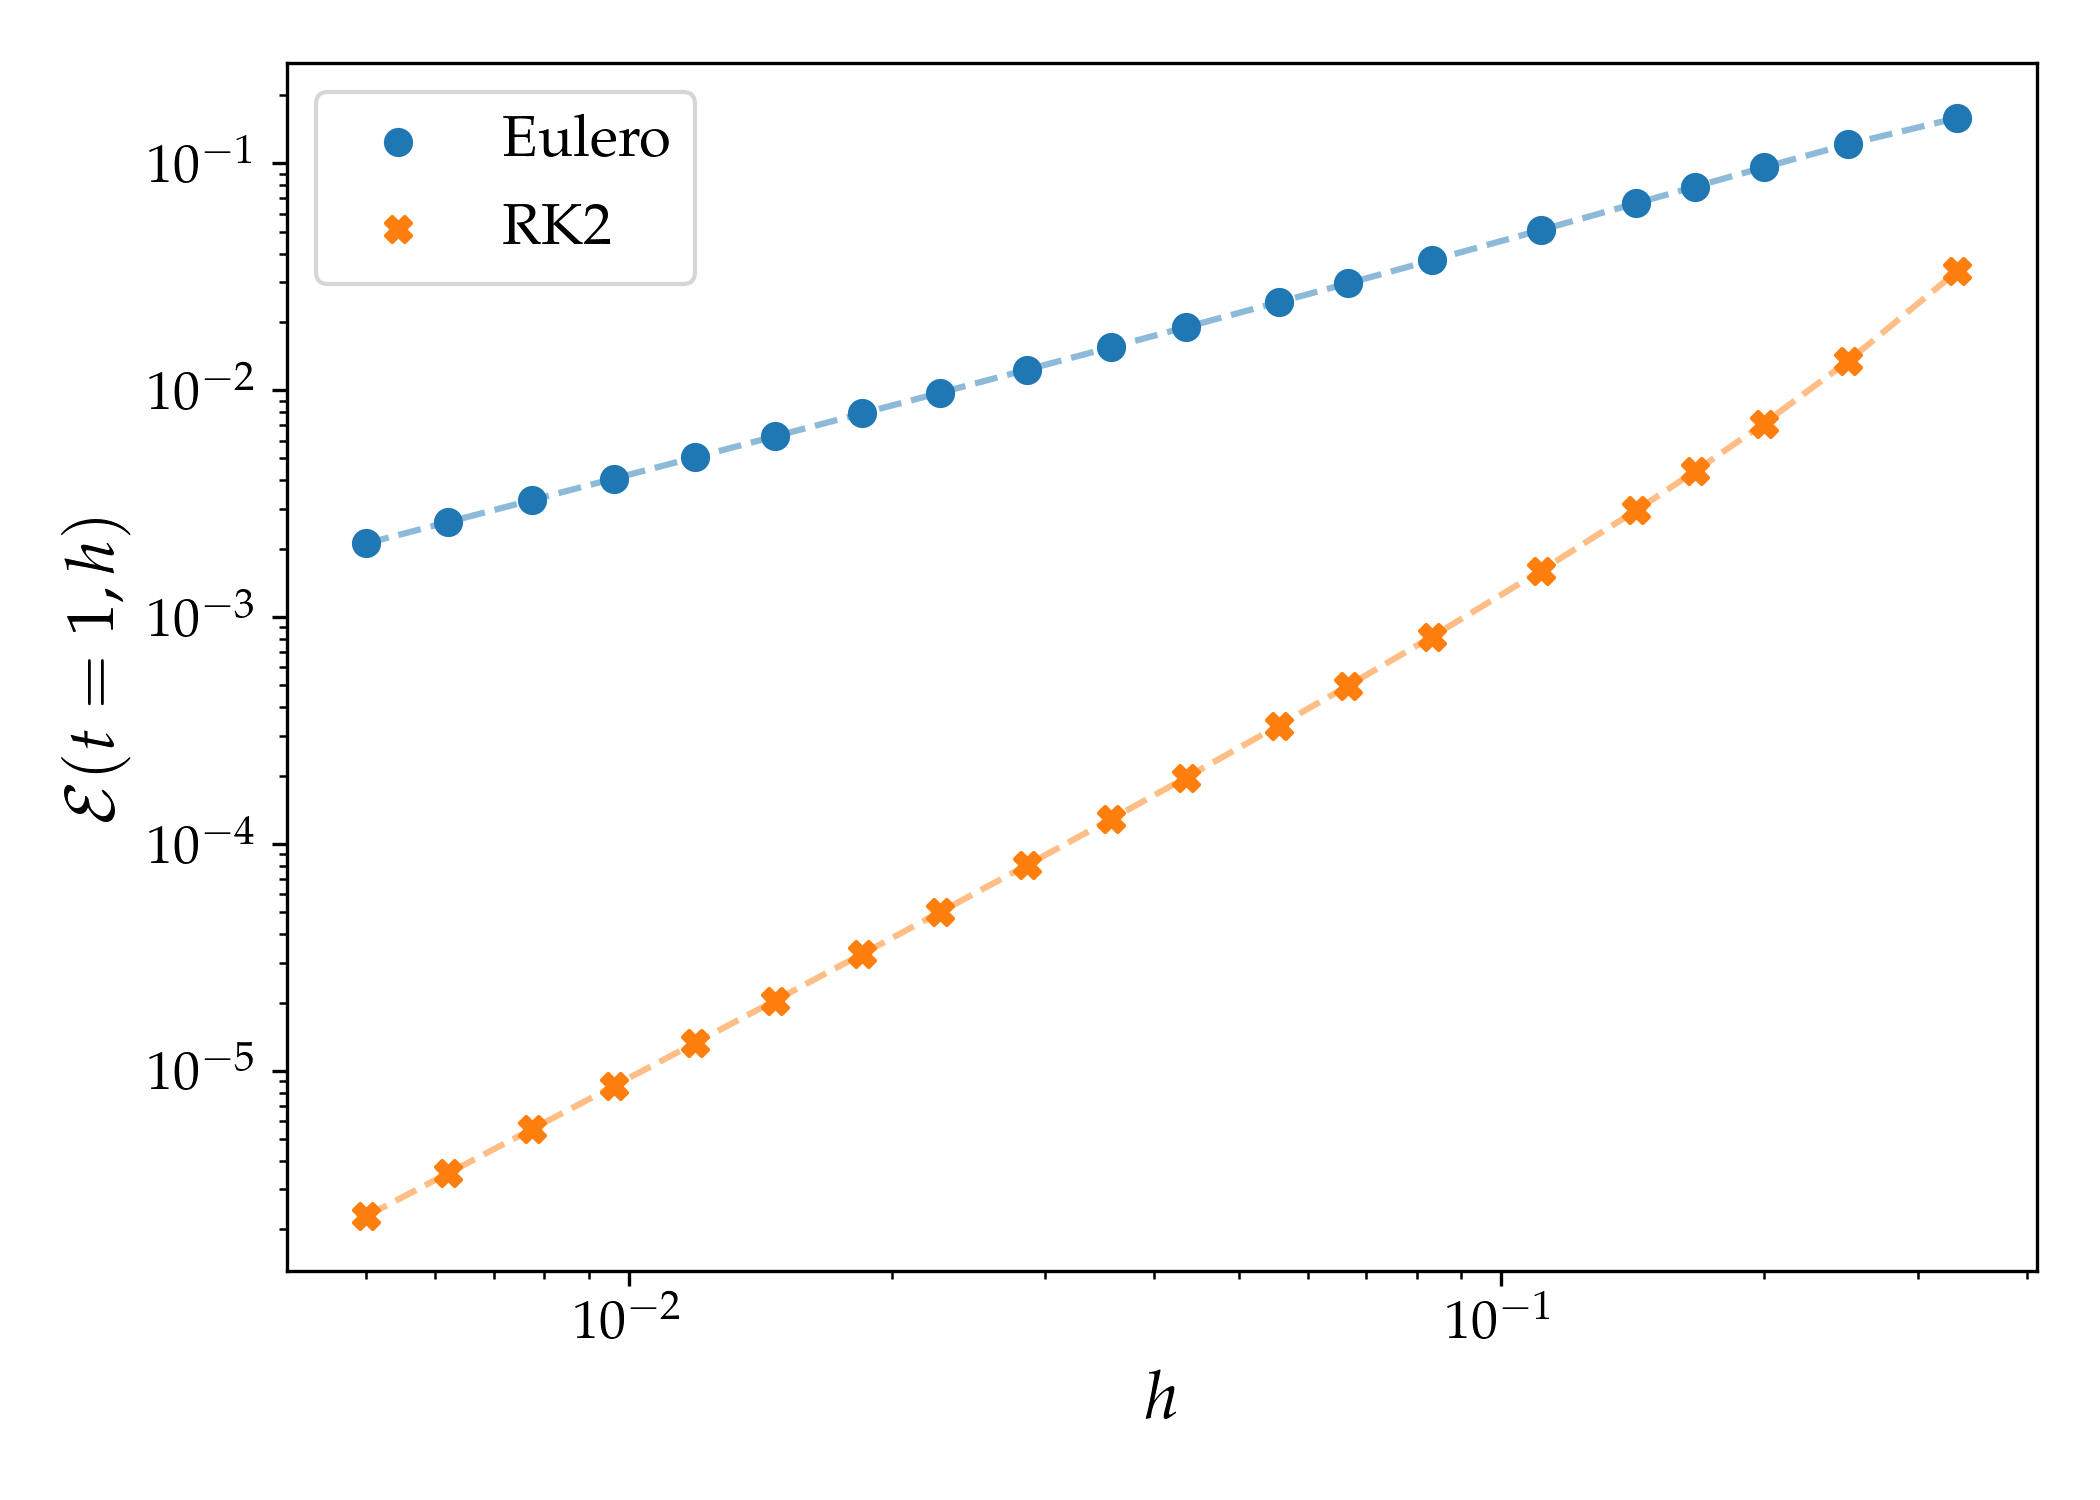
\includegraphics[width=0.7\linewidth]{images/17/scaling_confr.png}
    \caption{Confronto nello scaling dei singoli metodi. Si noti come la pendenza sia diversa, in particolare è maggiore per RK2: la sua convergenza è più rapida.}
    \label{fig: Scaling confr}
\end{figure}


\begin{figure}[H]
    \centering
    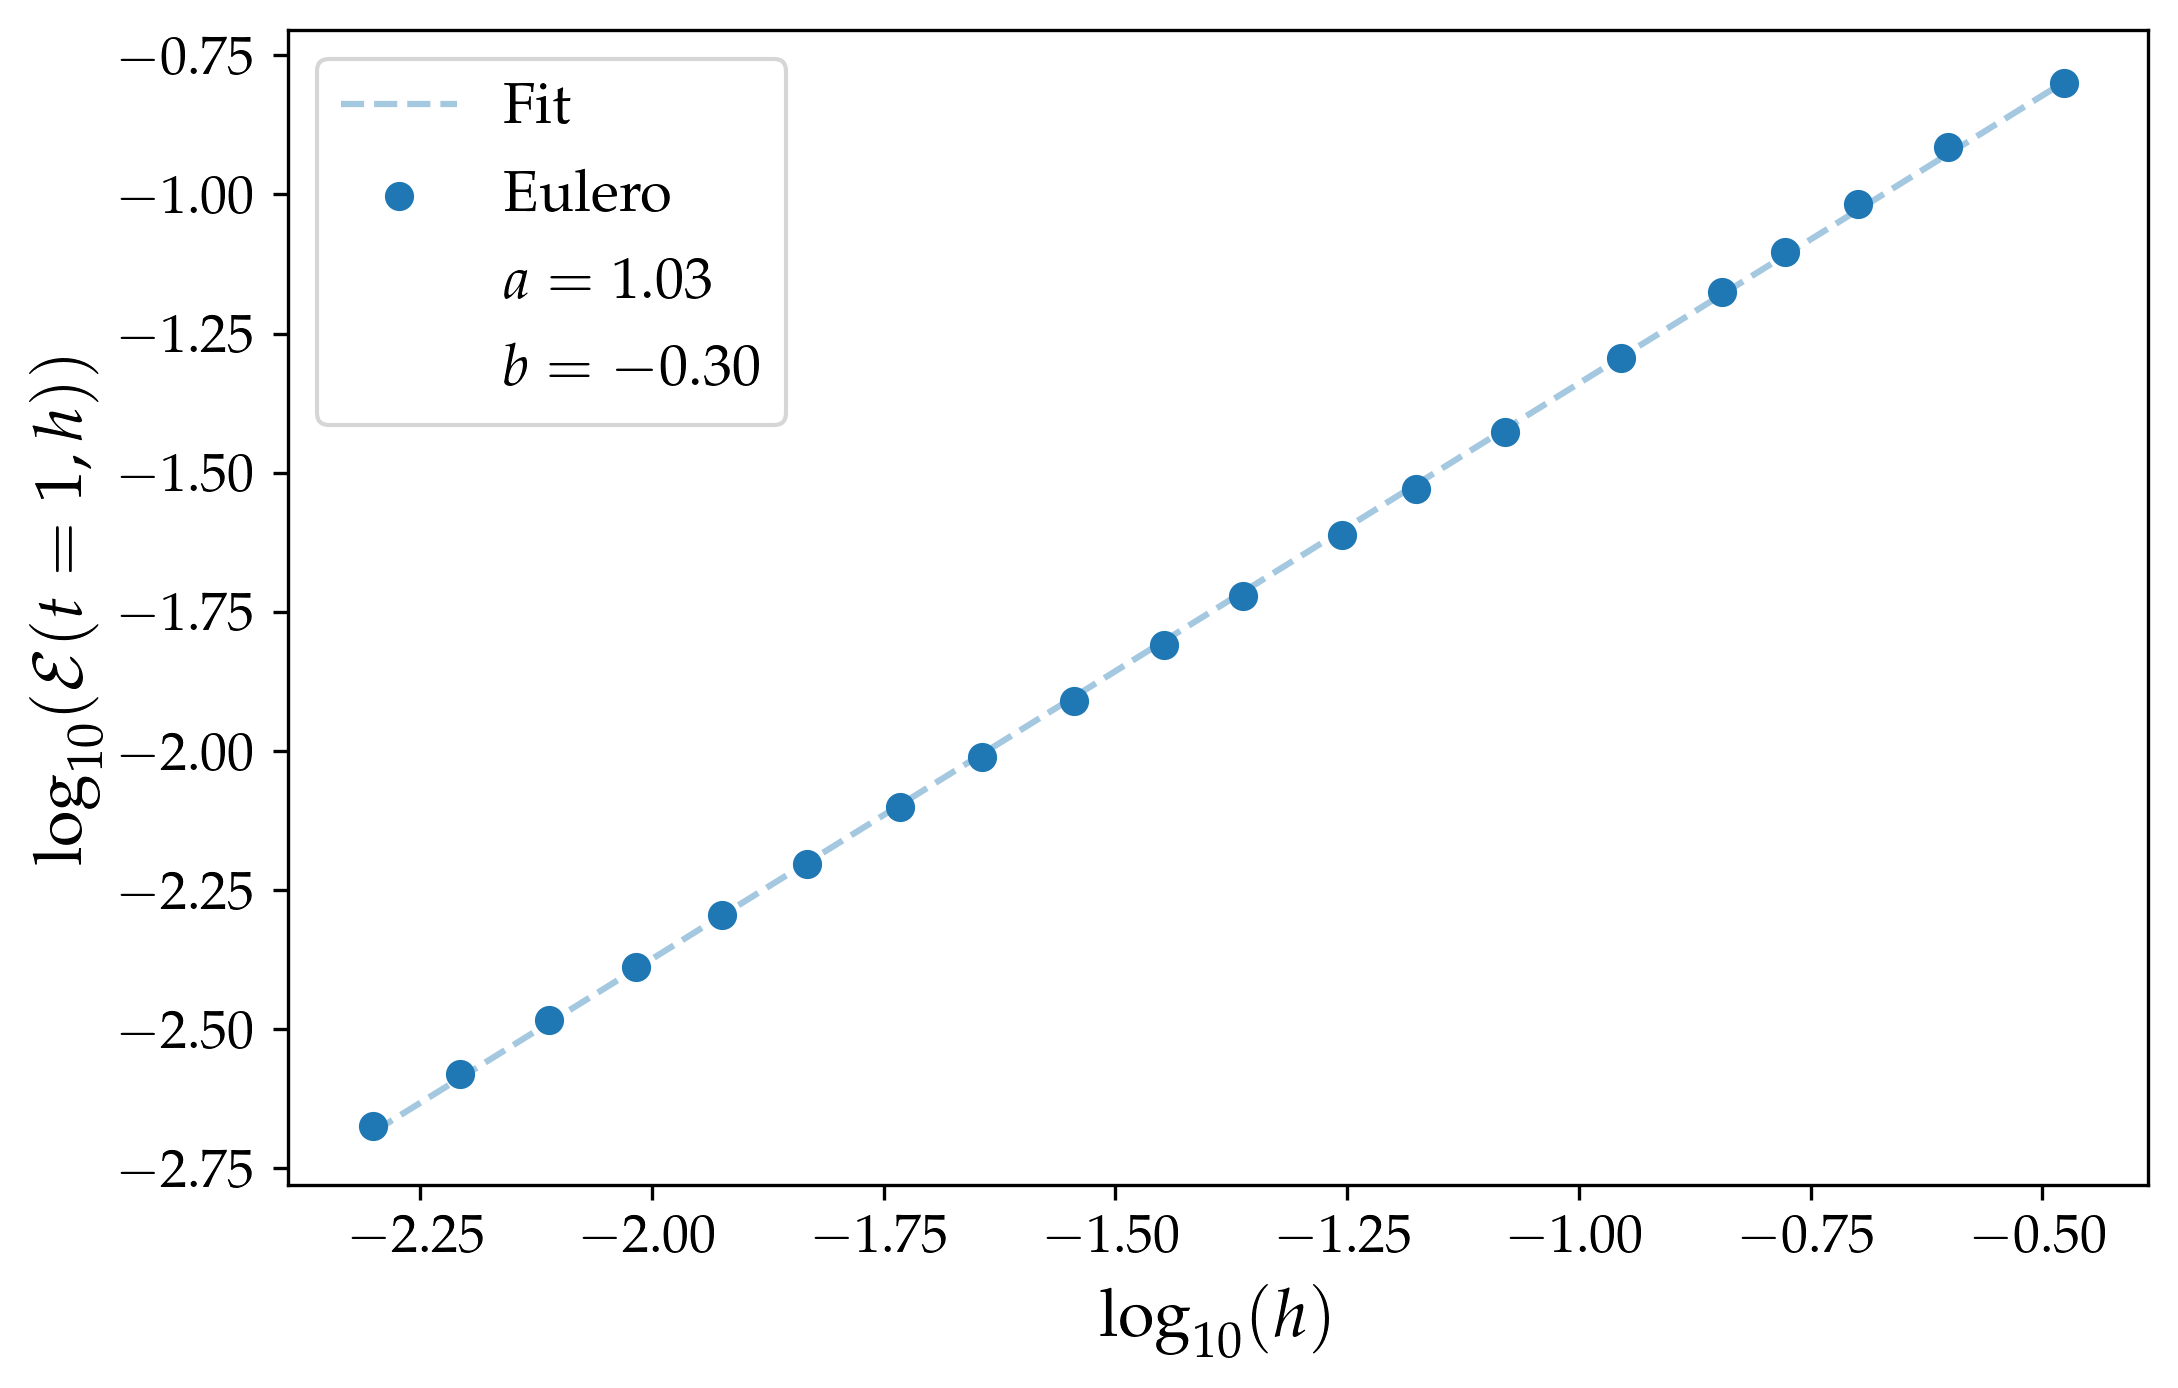
\includegraphics[width=0.8\linewidth]{images/17/fit_Eulero.png}
    \caption{Fit del metodo di Eulero: si verifica la convergenza lineare.}
    \label{fig: fit euler}
\end{figure}

\begin{figure}[H]
    \centering
    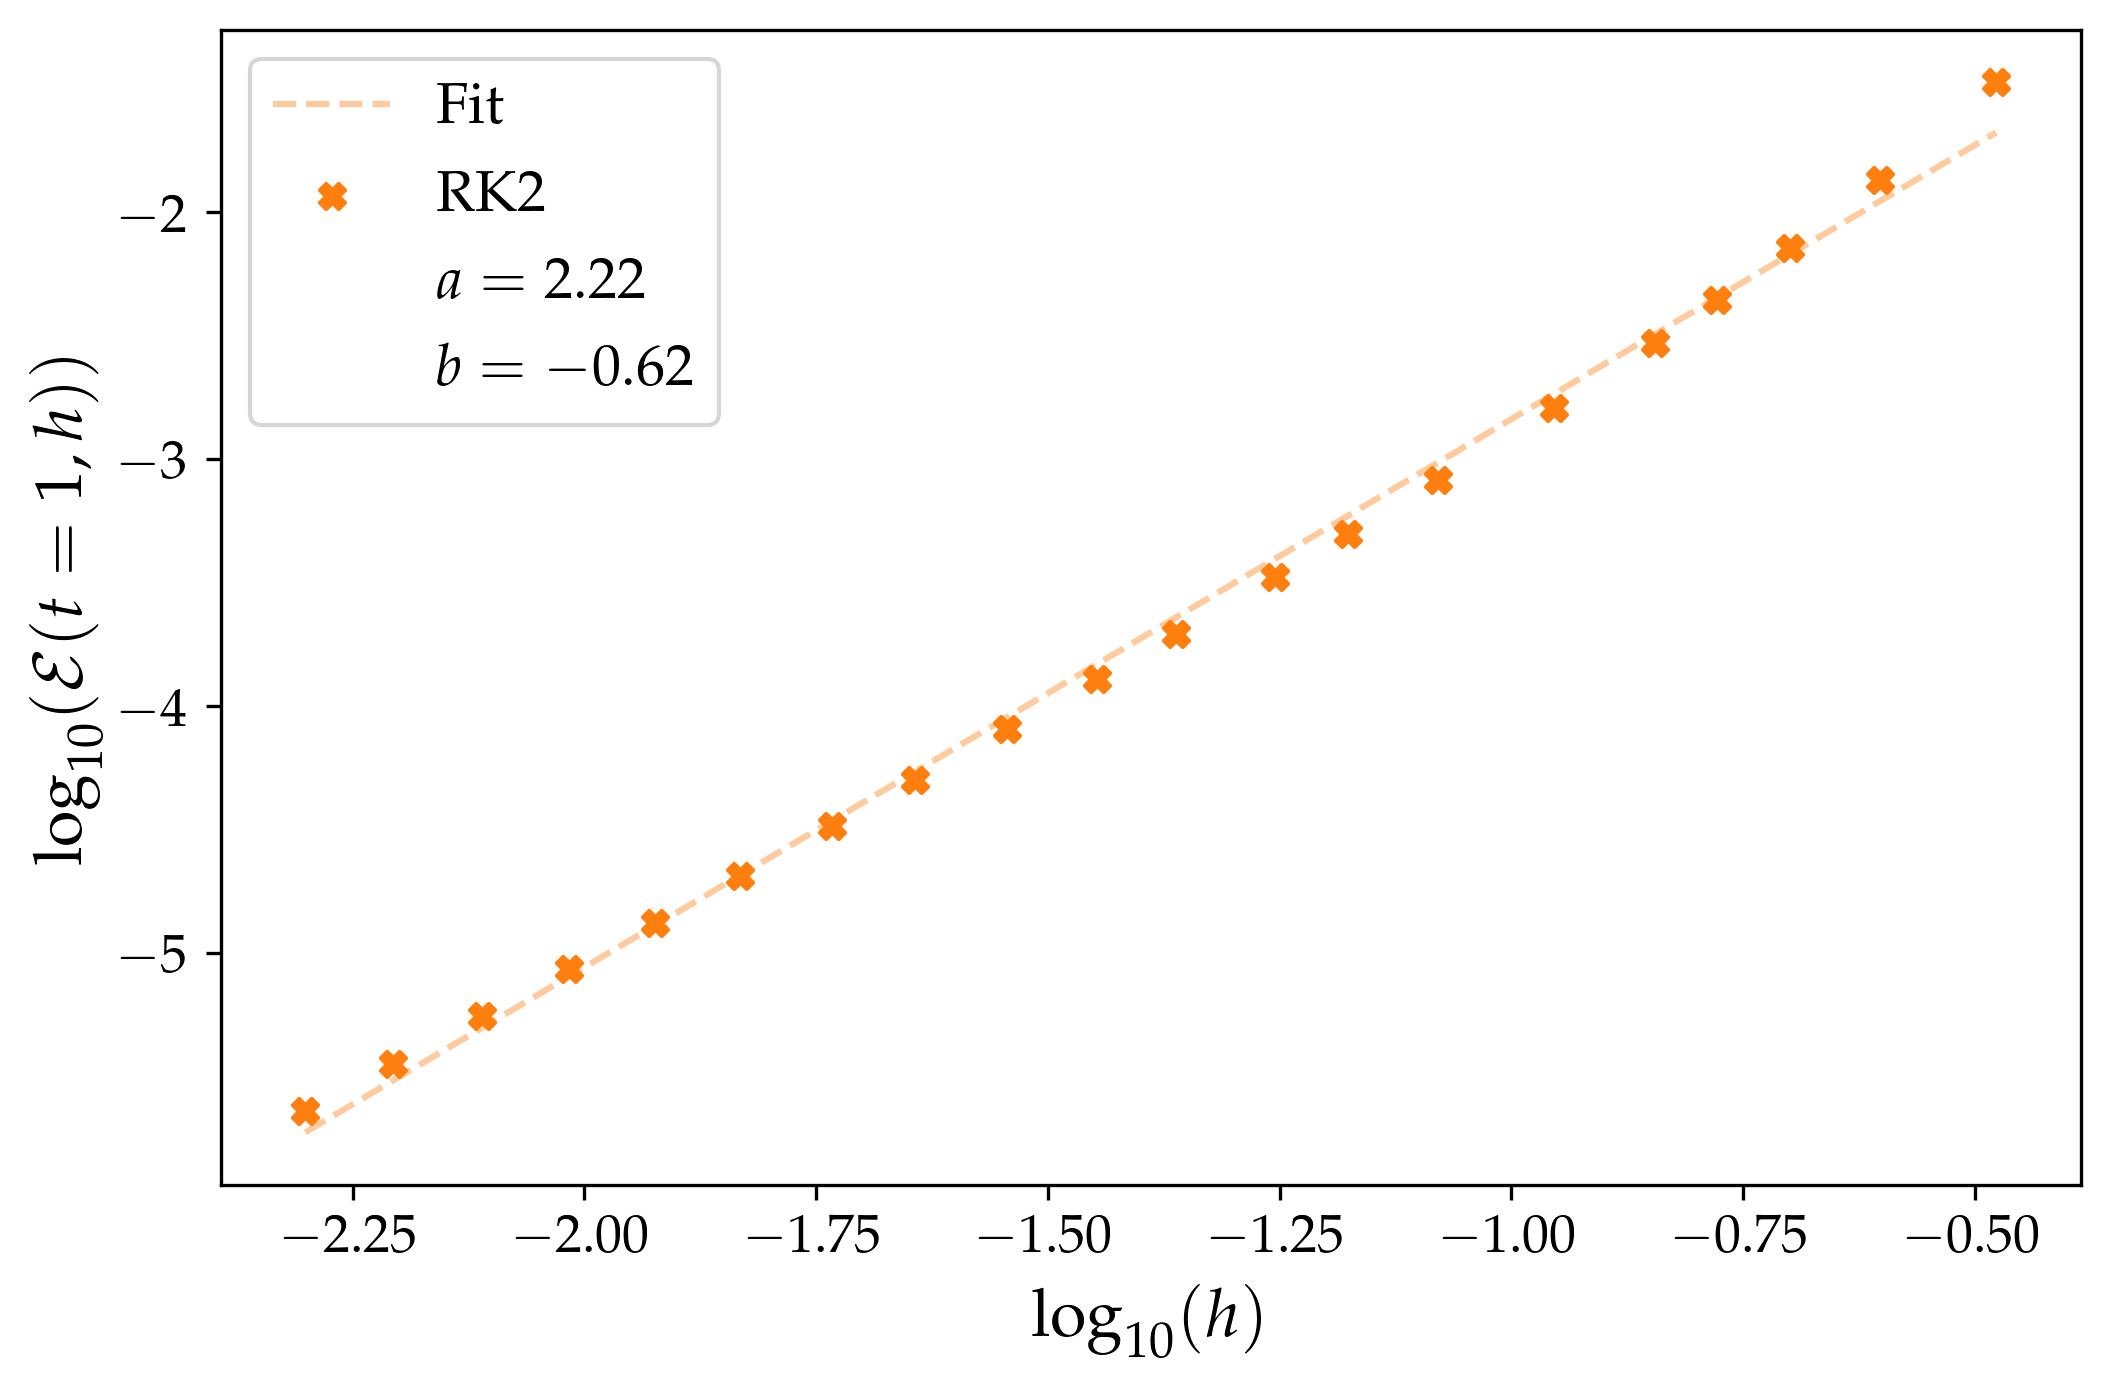
\includegraphics[width=0.8\linewidth]{images/17/fit_RK2.png}
    \caption{Fit del metodo RK2: si verifica la convergenza quadratica.}
    \label{fig: fit rk2}
\end{figure}

\newpage





\section{Esercizio 6.3.2}
\subsection{Problem Statement}

Considera l'equazione differenziale del pendolo senza l'approssimazione delle piccole oscillazioni, includendo un termine di attrito e un termine forzante:

\begin{equation*}
    \ddot{\theta}(t) = -\sin \theta - \gamma\dot{\theta}(t) + A \sin\left(\frac{2}{3}t\right)
\end{equation*}

con $A, \gamma \in (0, 2)$.

\noindent Risolvi numericamente l'equazione differenziale utilizzando il metodo RK4 e traccia i grafici di $\theta(t)$, $\dot{\theta}(t)$ e $\dot{\theta}(\theta)$ per i seguenti casi:

\begin{enumerate}
    \item $A = 0, \gamma = 0.3, 0.6, 0.9$
    \item $A = 0.5, 1.5, \gamma = 0.3, 0.9$
\end{enumerate}

\noindent Dimostra che l'algoritmo è di ordine 4.

\subsection{Premessa Teorica}
L'algoritmo a cui abbiamo accennato e che abbiamo studiato nell'esercizio precedente, RK2, appartiene alla famiglia dei metodi di Runge–Kutta. Tra questi, uno dei più utilizzati è il metodo RK4, che possiede ordine globale quattro: Analizzeremo quindi la soluzione del pendolo con forzante e smorzante usando RK4 per la risoluzione dell'ODE.


\subsection{Metodi Numerici e Algoritmi}

La definizione dell'algoritmo è:
\[
\eta(x+ h,h) = \eta(x,h) + \frac{h}{6} \left( k_1 + 2k_2 + 2k_3 + k_4 \right)
\]
\begin{align*}
    k_1 &= f(x, y) , \\
    k_2 &= f(x + \frac{1}{2}h, y + \frac{1}{2}hk_1) , \\
    k_3 &= f(x + \frac{1}{2}h, y + \frac{1}{2}hk_2) , \\
    k_4 &= f(x + h, y + hk_3) .
\end{align*}

\bigskip\noindent
Si può dimostrare che il metodo così descritto ha ordine di convergenza (globale) 4.

\subsection{Risultati e Discussione}

Desidero mostrare alcune figure che mettono in risalto i comportamenti particolari delle soluzioni di questo sistema fisico: variare i parametri $A$ e $\gamma$ equivale a modificare il fenomeno e i risultati sono visibili nei plot e nelle animazioni che propongo.\\
In Fig.\ref{fig: A0_g03} - \ref{fig: A0_g09} si trovano i diagrammi di $\theta(t)$, $\dot \theta(t)$, e $\dot\theta(\theta)$ con $A=0, \gamma\in[0.3, 0.6, 0.9]$. Qui viene azzerato il termine forzante, osserviamo solo lo smorzamento. Nel diagramma delle fasi la presenza dell'attrito è evidenziata dal fatto che la traiettoria non si chiude ma spiraleggia verso il punto di equilibrio, a causa della progressiva dissipazione di energia.\\
A seguire, in Fig. \ref{fig: A05_g03} - \ref{fig: A05_g09} l'esempio dell'introduzione di una forzante poco intensa; in Fig. \ref{fig: A15_g03} - \ref{fig: A15_g09} una più intensa.

\medskip\noindent
Infine alcune animazioni che rendono chiara la più semplice delle interpretazioni del problema rappresentato dall'ODE: un pendolo con lunghezza unitaria oscilla seguendo le soluzioni delle equazioni differenziali che abbiamo risolto con RK4. Il link a \url{https://github.com/mvolpato-unimib/Lab_comp/tree/main/ex17/anim}.

\url{}




\begin{figure}[H]
    \centering
    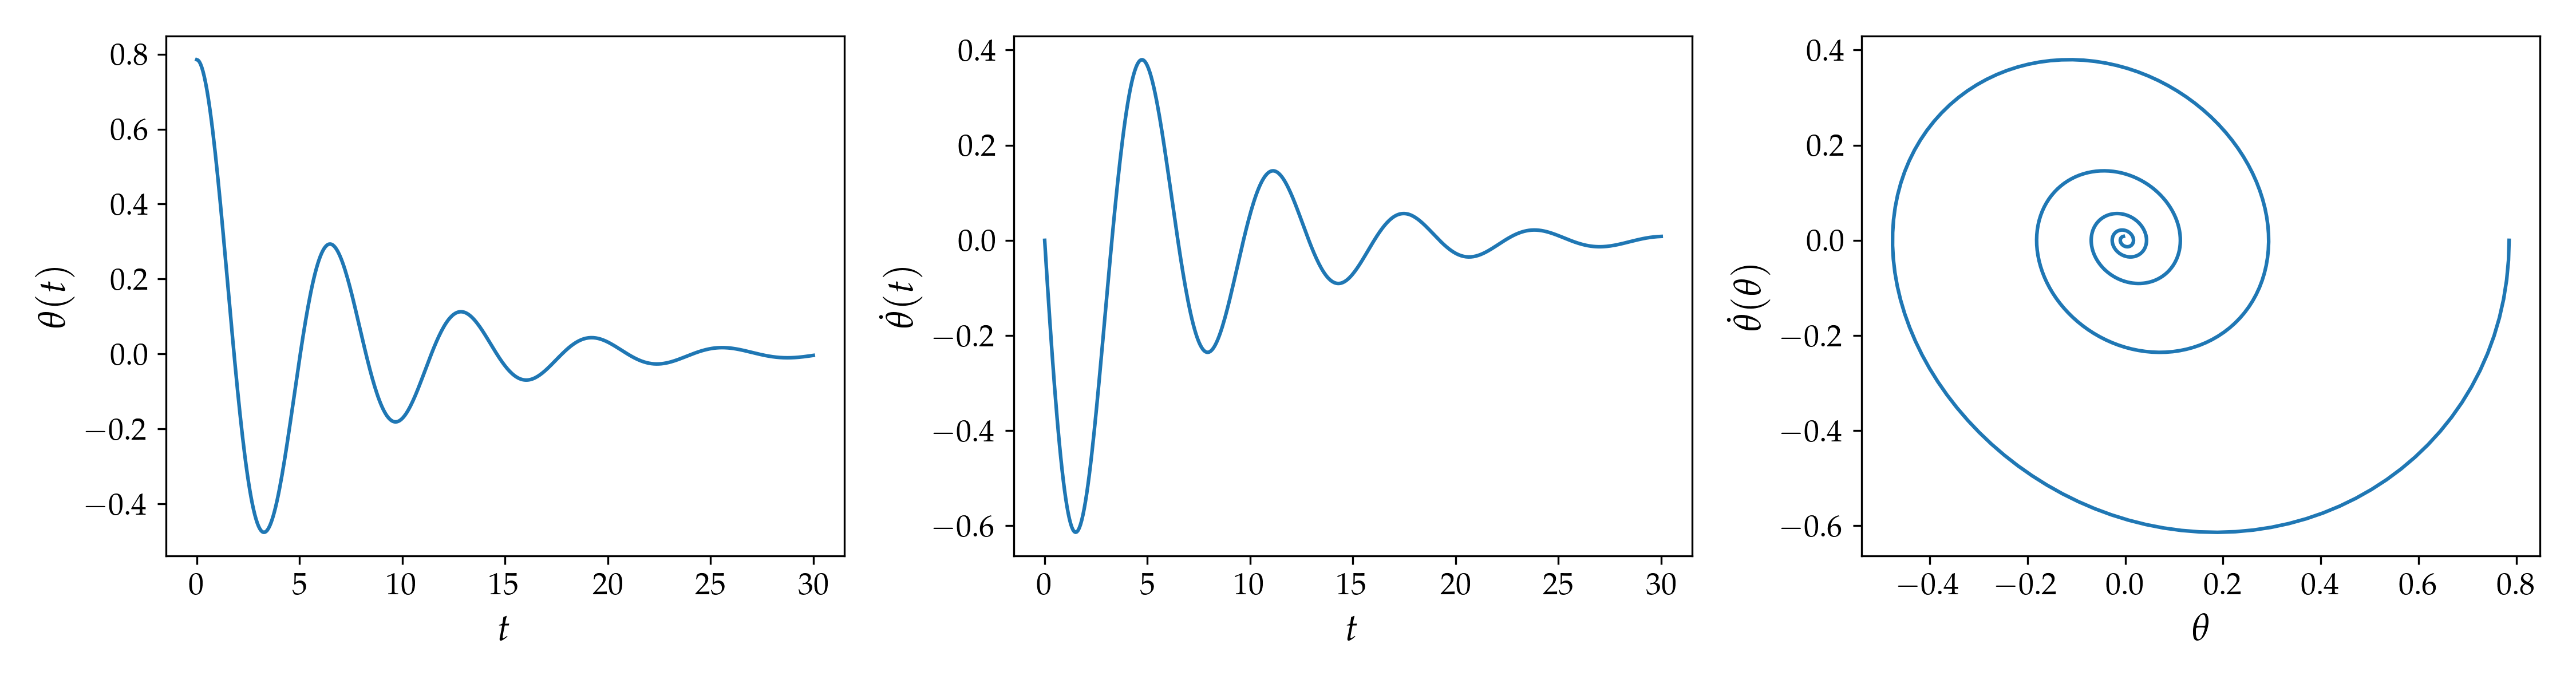
\includegraphics[width=\linewidth]{images/17/17 - 2/A0_g03.png}
    \caption{$A=0, \gamma=0.3$}
    \label{fig: A0_g03}
\end{figure}


\begin{figure}[H]
    \centering
    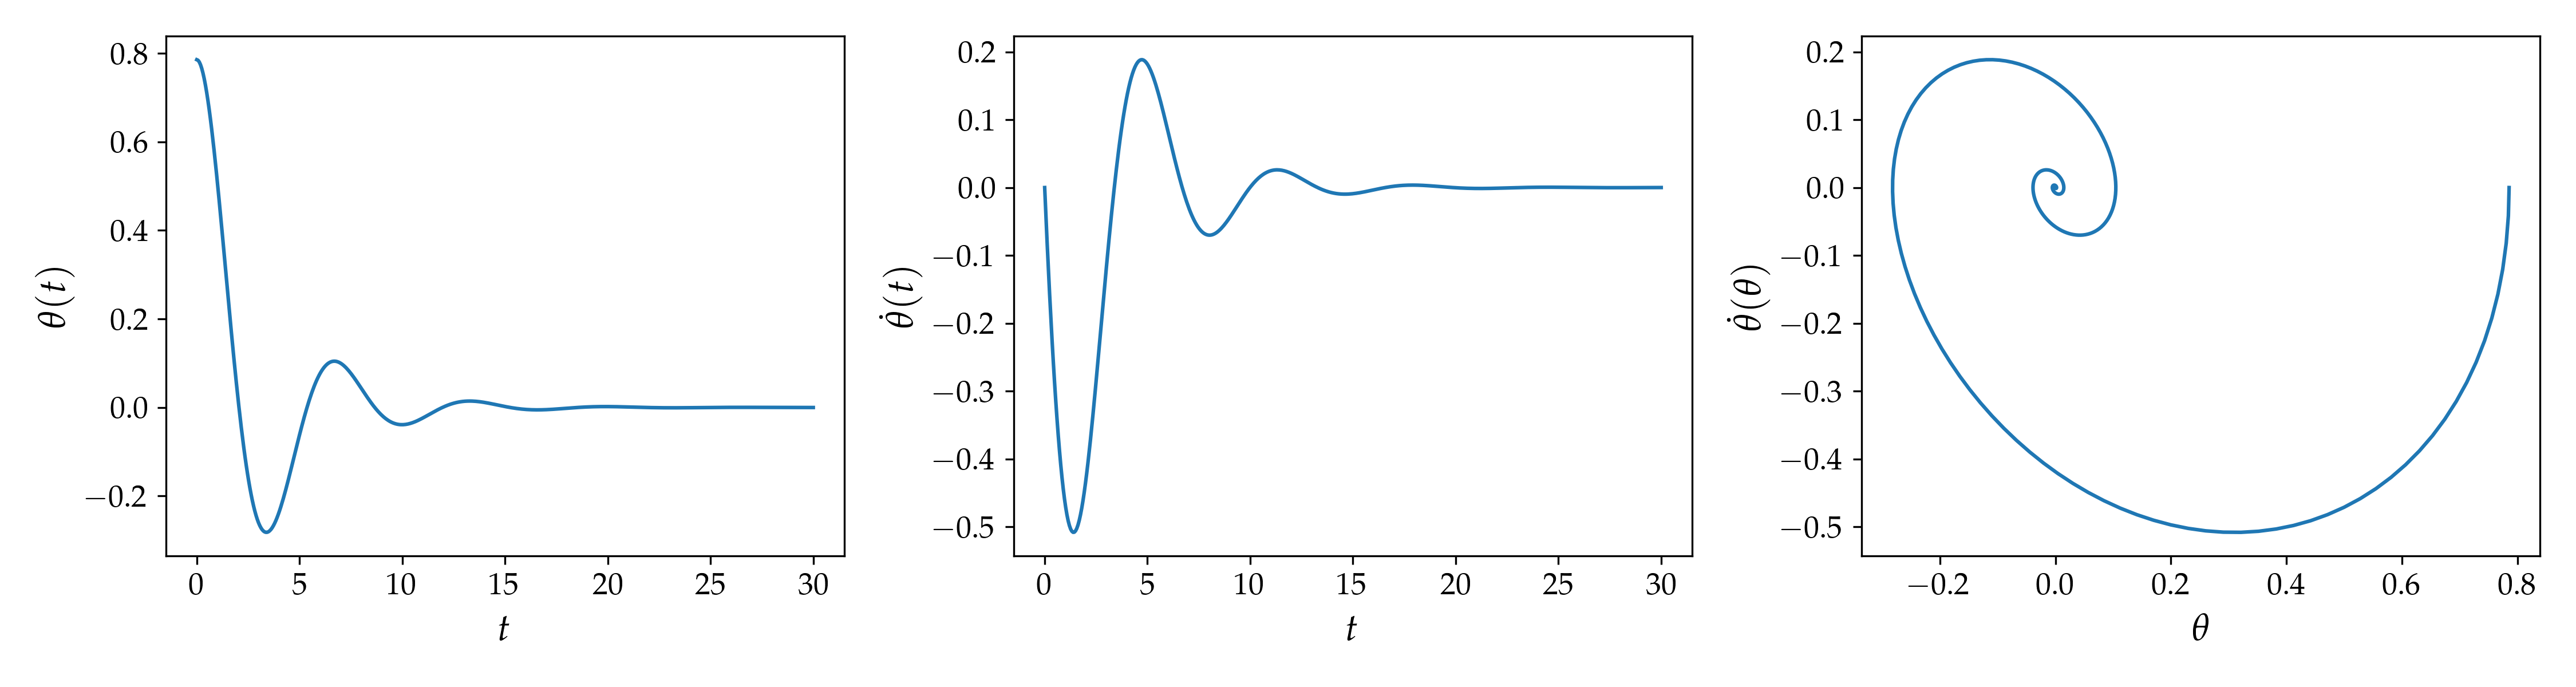
\includegraphics[width=\linewidth]{images/17/17 - 2/A0_g06.png}
    \caption{$A=0, \gamma=0.6$}
    \label{fig: A0_g06}
\end{figure}


\begin{figure}[H]
    \centering
    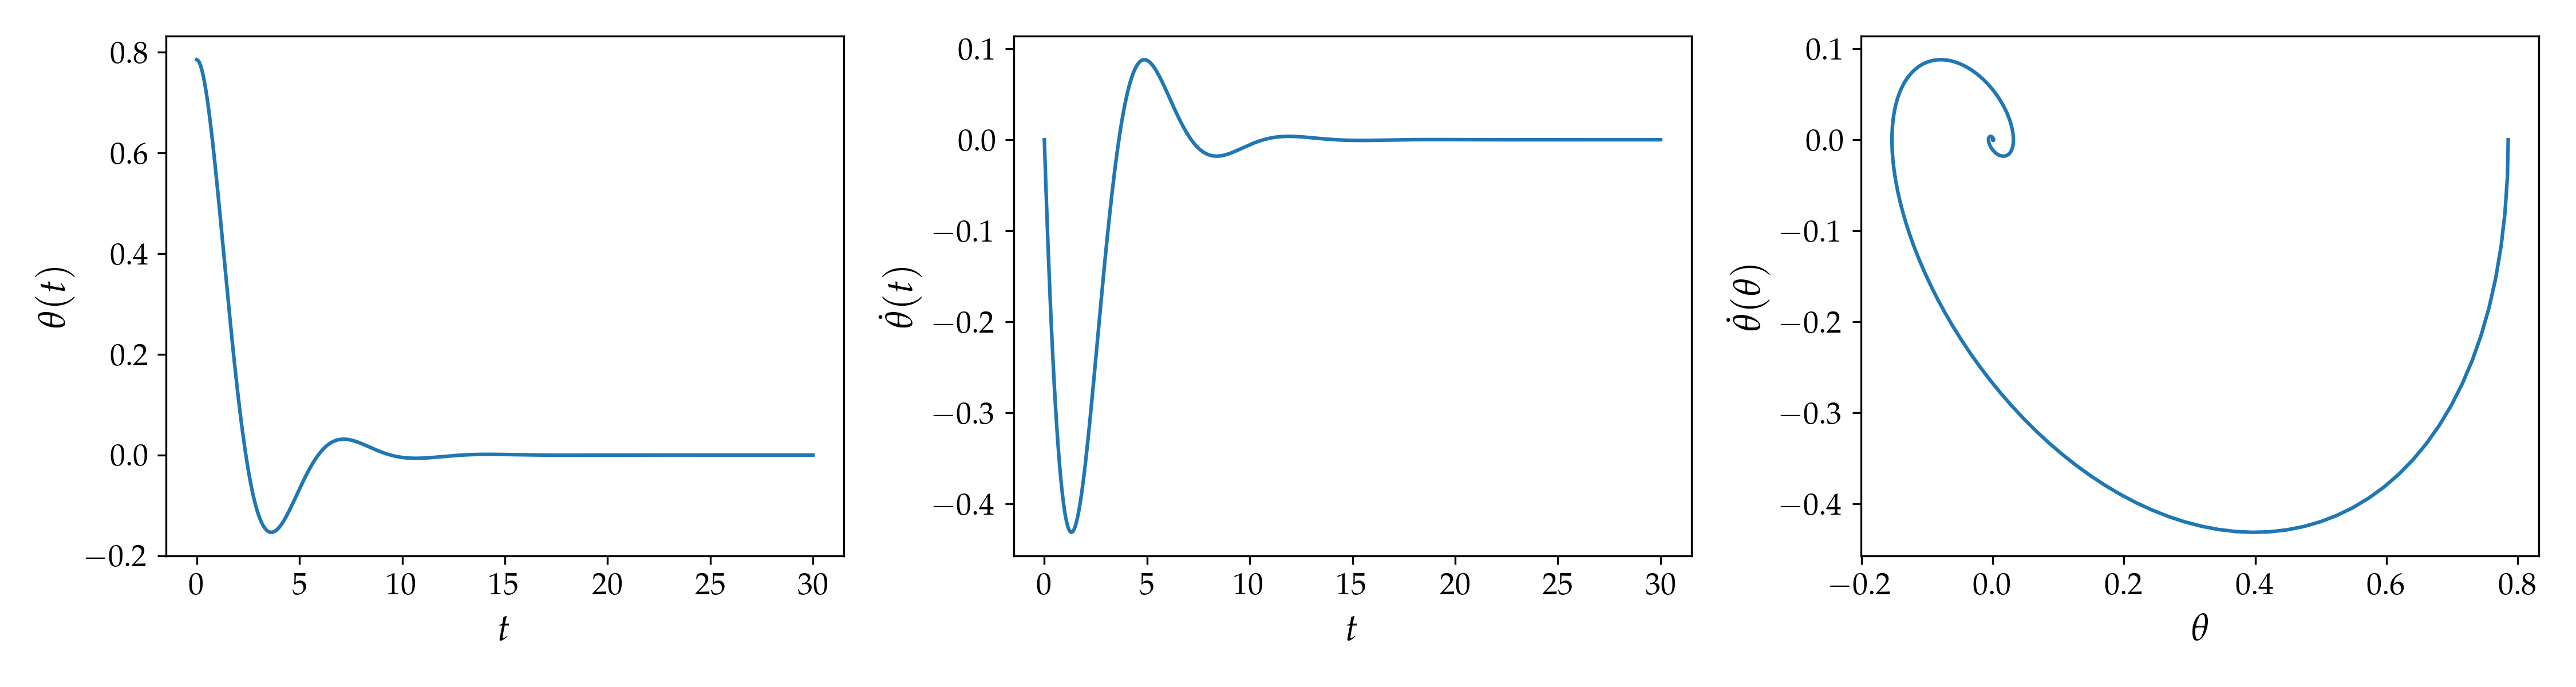
\includegraphics[width=\linewidth]{images/17/17 - 2/A0_g09.png}
    \caption{$A=0, \gamma=0.9$}
    \label{fig: A0_g09}
\end{figure}

\newpage

\begin{figure}[H]
    \centering
    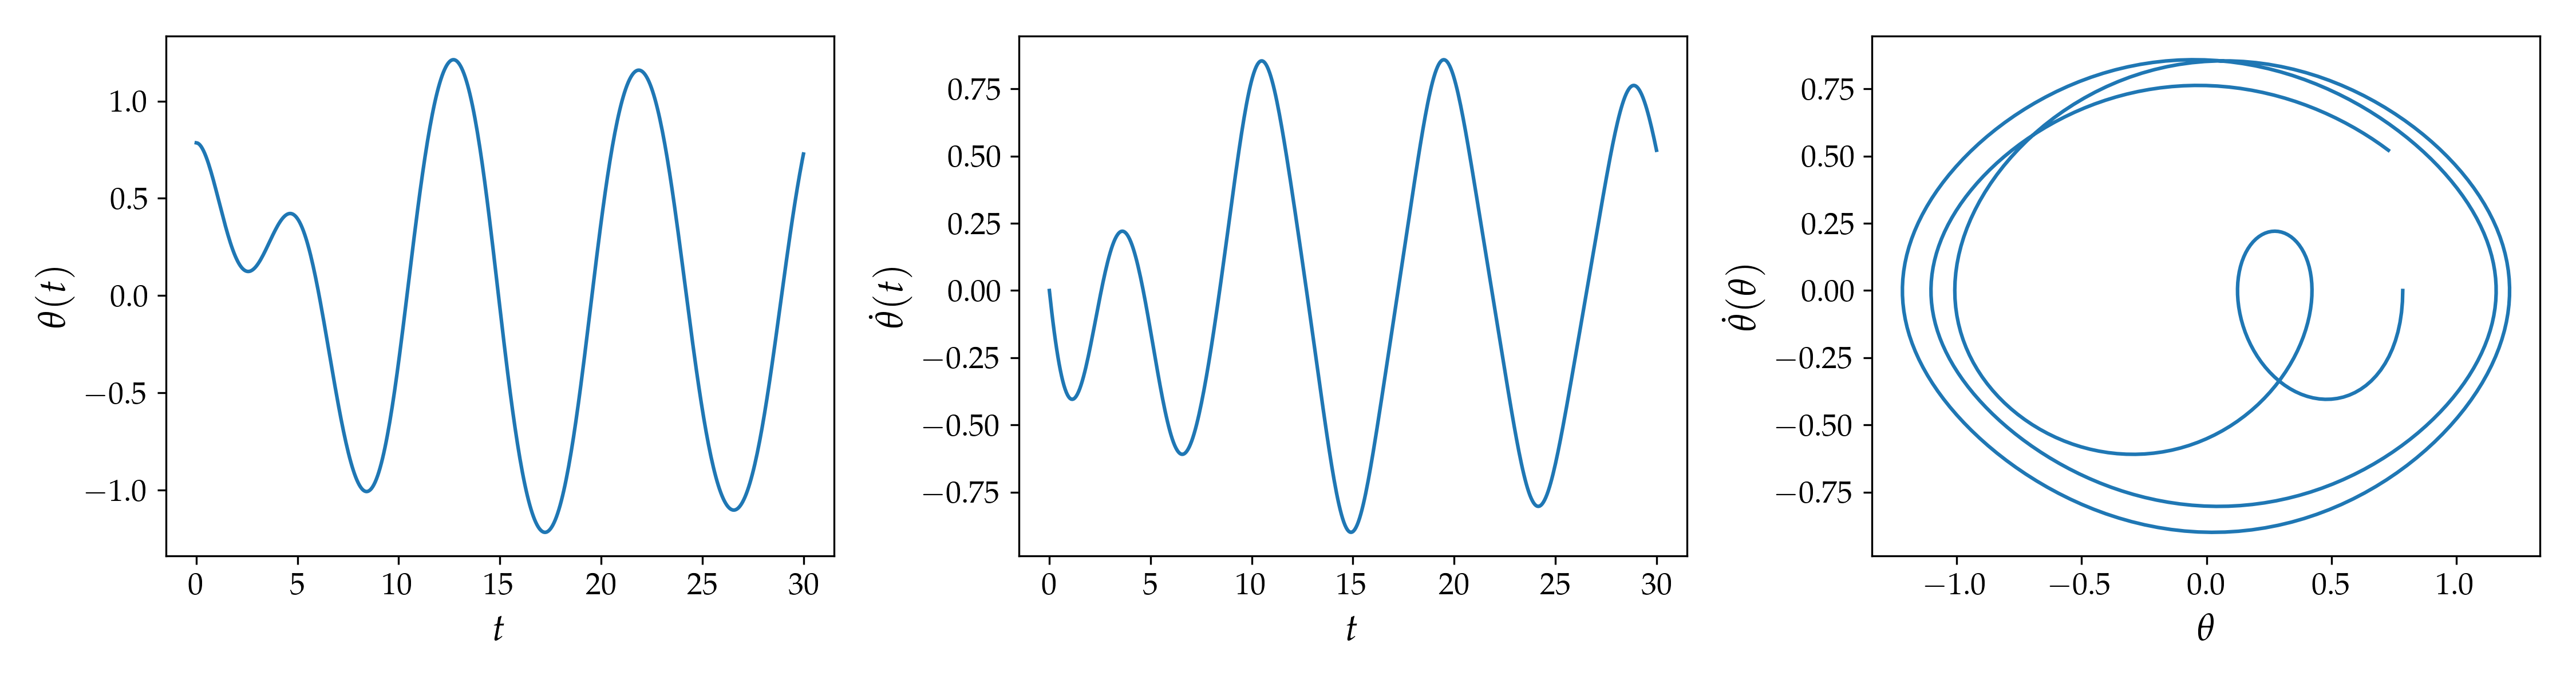
\includegraphics[width=\linewidth]{images/17/17 - 2/A05_g03.png}
    \caption{$A=0.5, \gamma=0.3$}
    \label{fig: A05_g03}
\end{figure}


\begin{figure}[H]
    \centering
    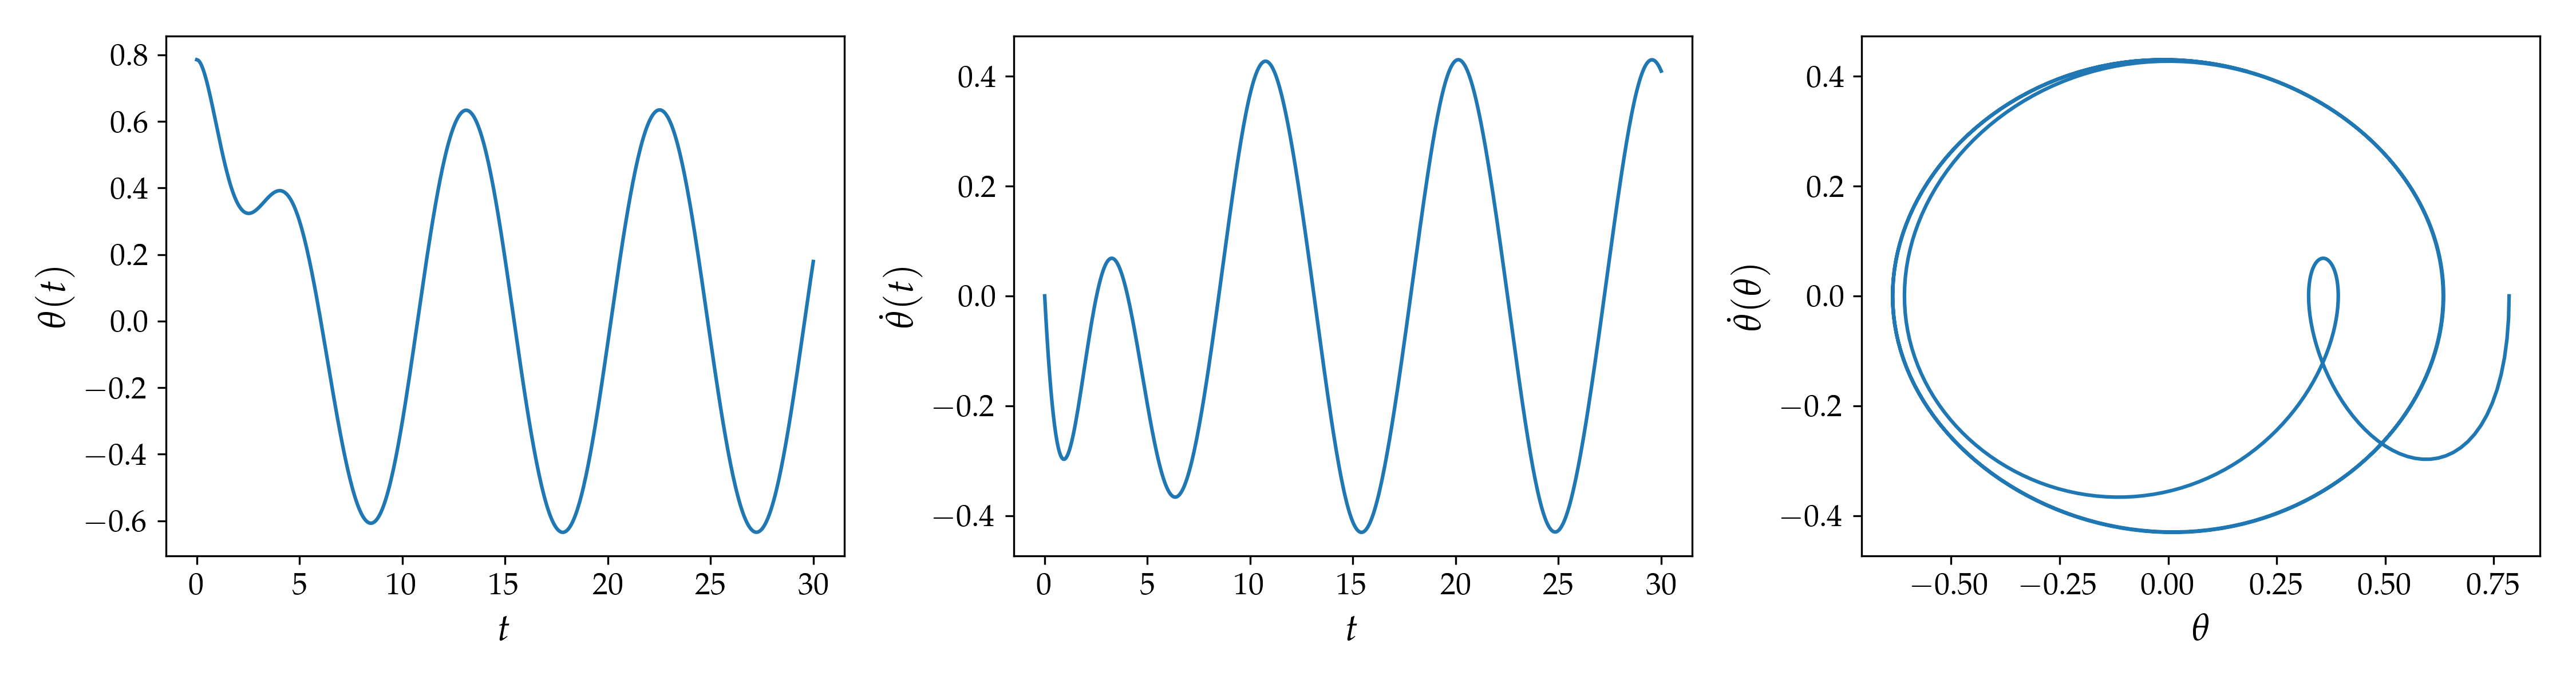
\includegraphics[width=\linewidth]{images/17/17 - 2/A05_g09.png}
    \caption{$A=0.5, \gamma=0.9$}
    \label{fig: A05_g09}
\end{figure}



\begin{figure}[H]
    \centering
    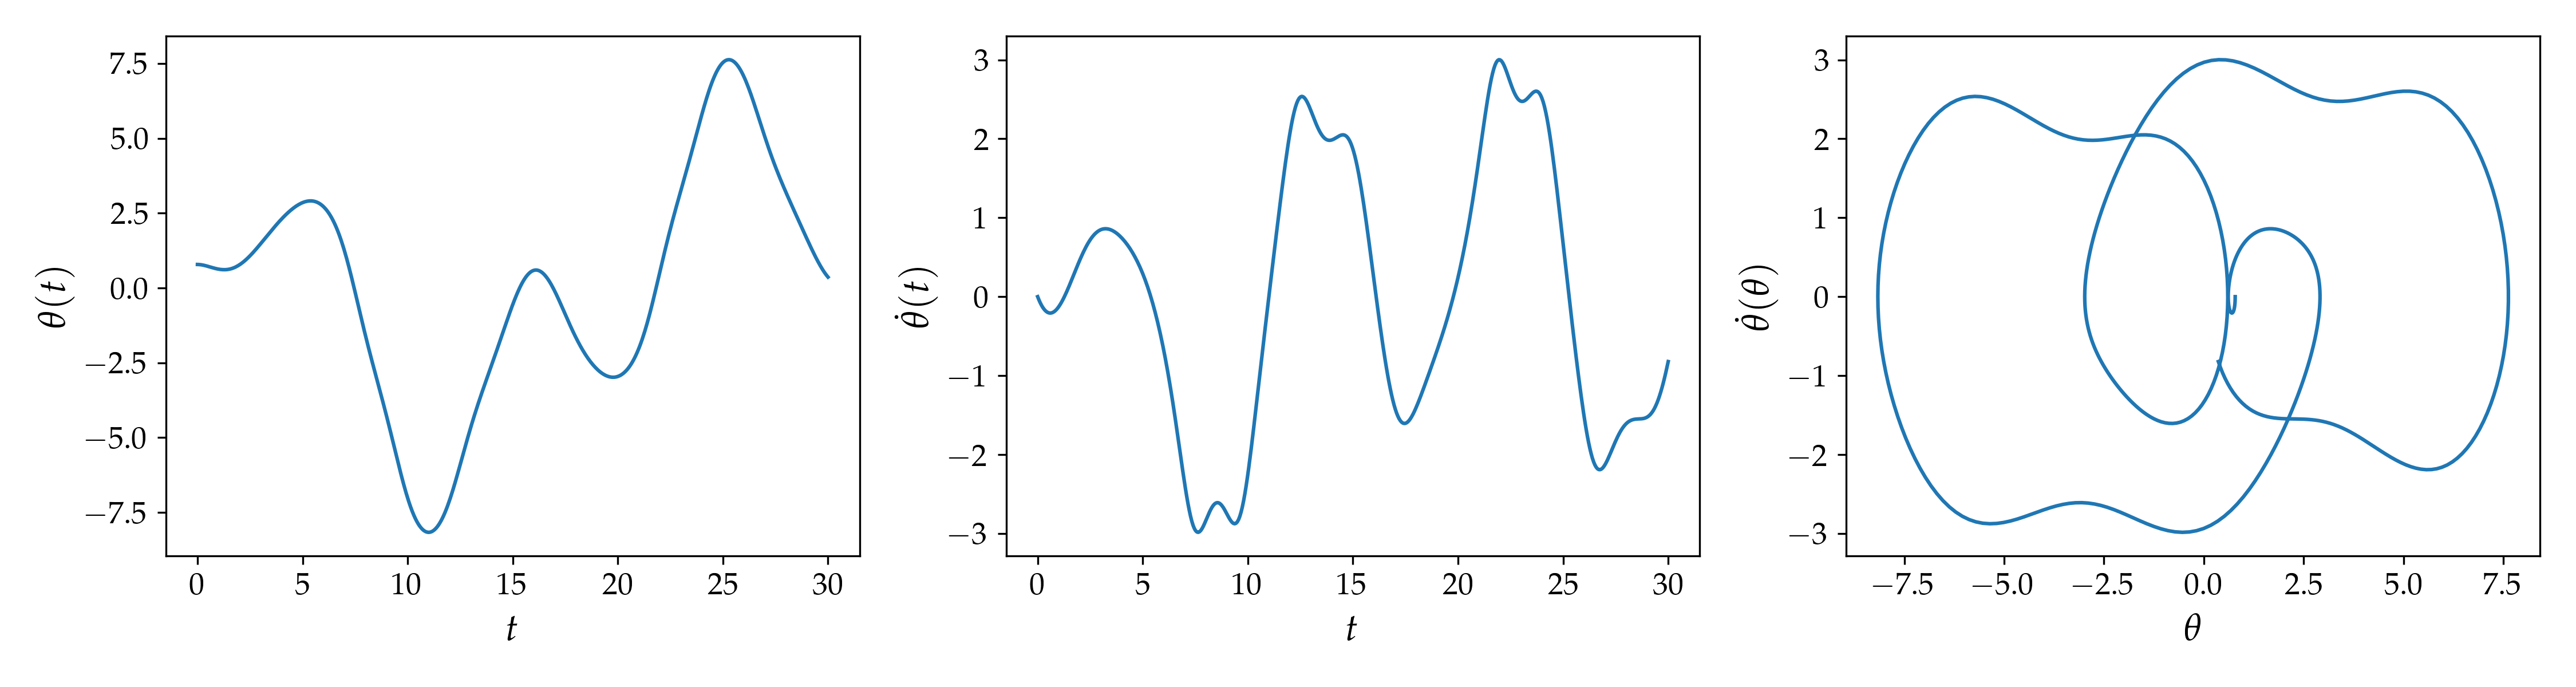
\includegraphics[width=\linewidth]{images/17/17 - 2/A15_g03.png}
    \caption{$A=1.5, \gamma=0.3$}
    \label{fig: A15_g03}
\end{figure}


\begin{figure}[H]
    \centering
    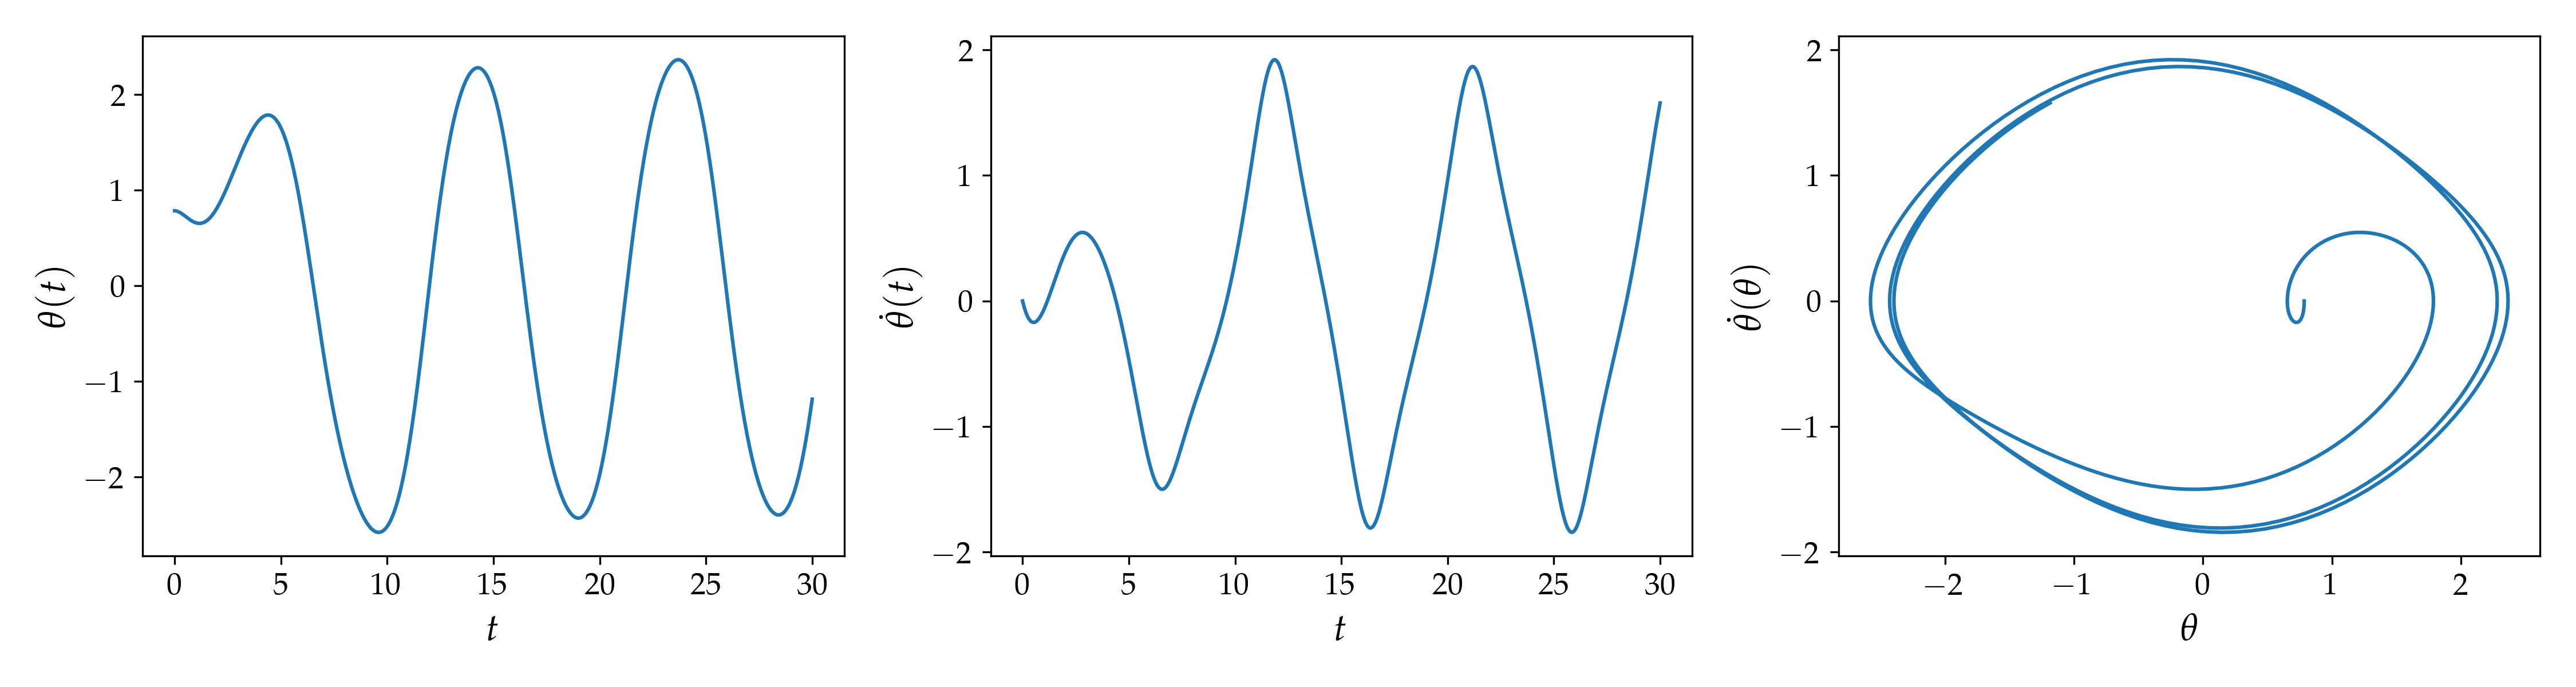
\includegraphics[width=\linewidth]{images/17/17 - 2/A15_g09.png}
    \caption{$A=1.5, \gamma=0.9$}
    \label{fig: A15_g09}
\end{figure}

\noindent Infine procediamo con la valutazione dell'ordine di convergenza del metodo; in particolare con un fit lineare dimostriamo che questo ha scaling di ordine 4.\\
Fissando uno dei diversi casi di indagine come test, si sceglie $A=0, \gamma=0.3$, e un tempo per confrontare le soluzioni al variare solo del passo $h$, scegliamo $t=1$:\\
di seguito la Fig. \ref{fig: fit_rk4} in cui risulta che 
\begin{align*}
    \log_{10}(\mathcal{E(h)}) &\approx a\cdot \log_{10}(h)\\
    \mathcal{E(h)} &\approx h^a, \quad a=4.30
\end{align*}


\begin{figure}[H]
    \centering
    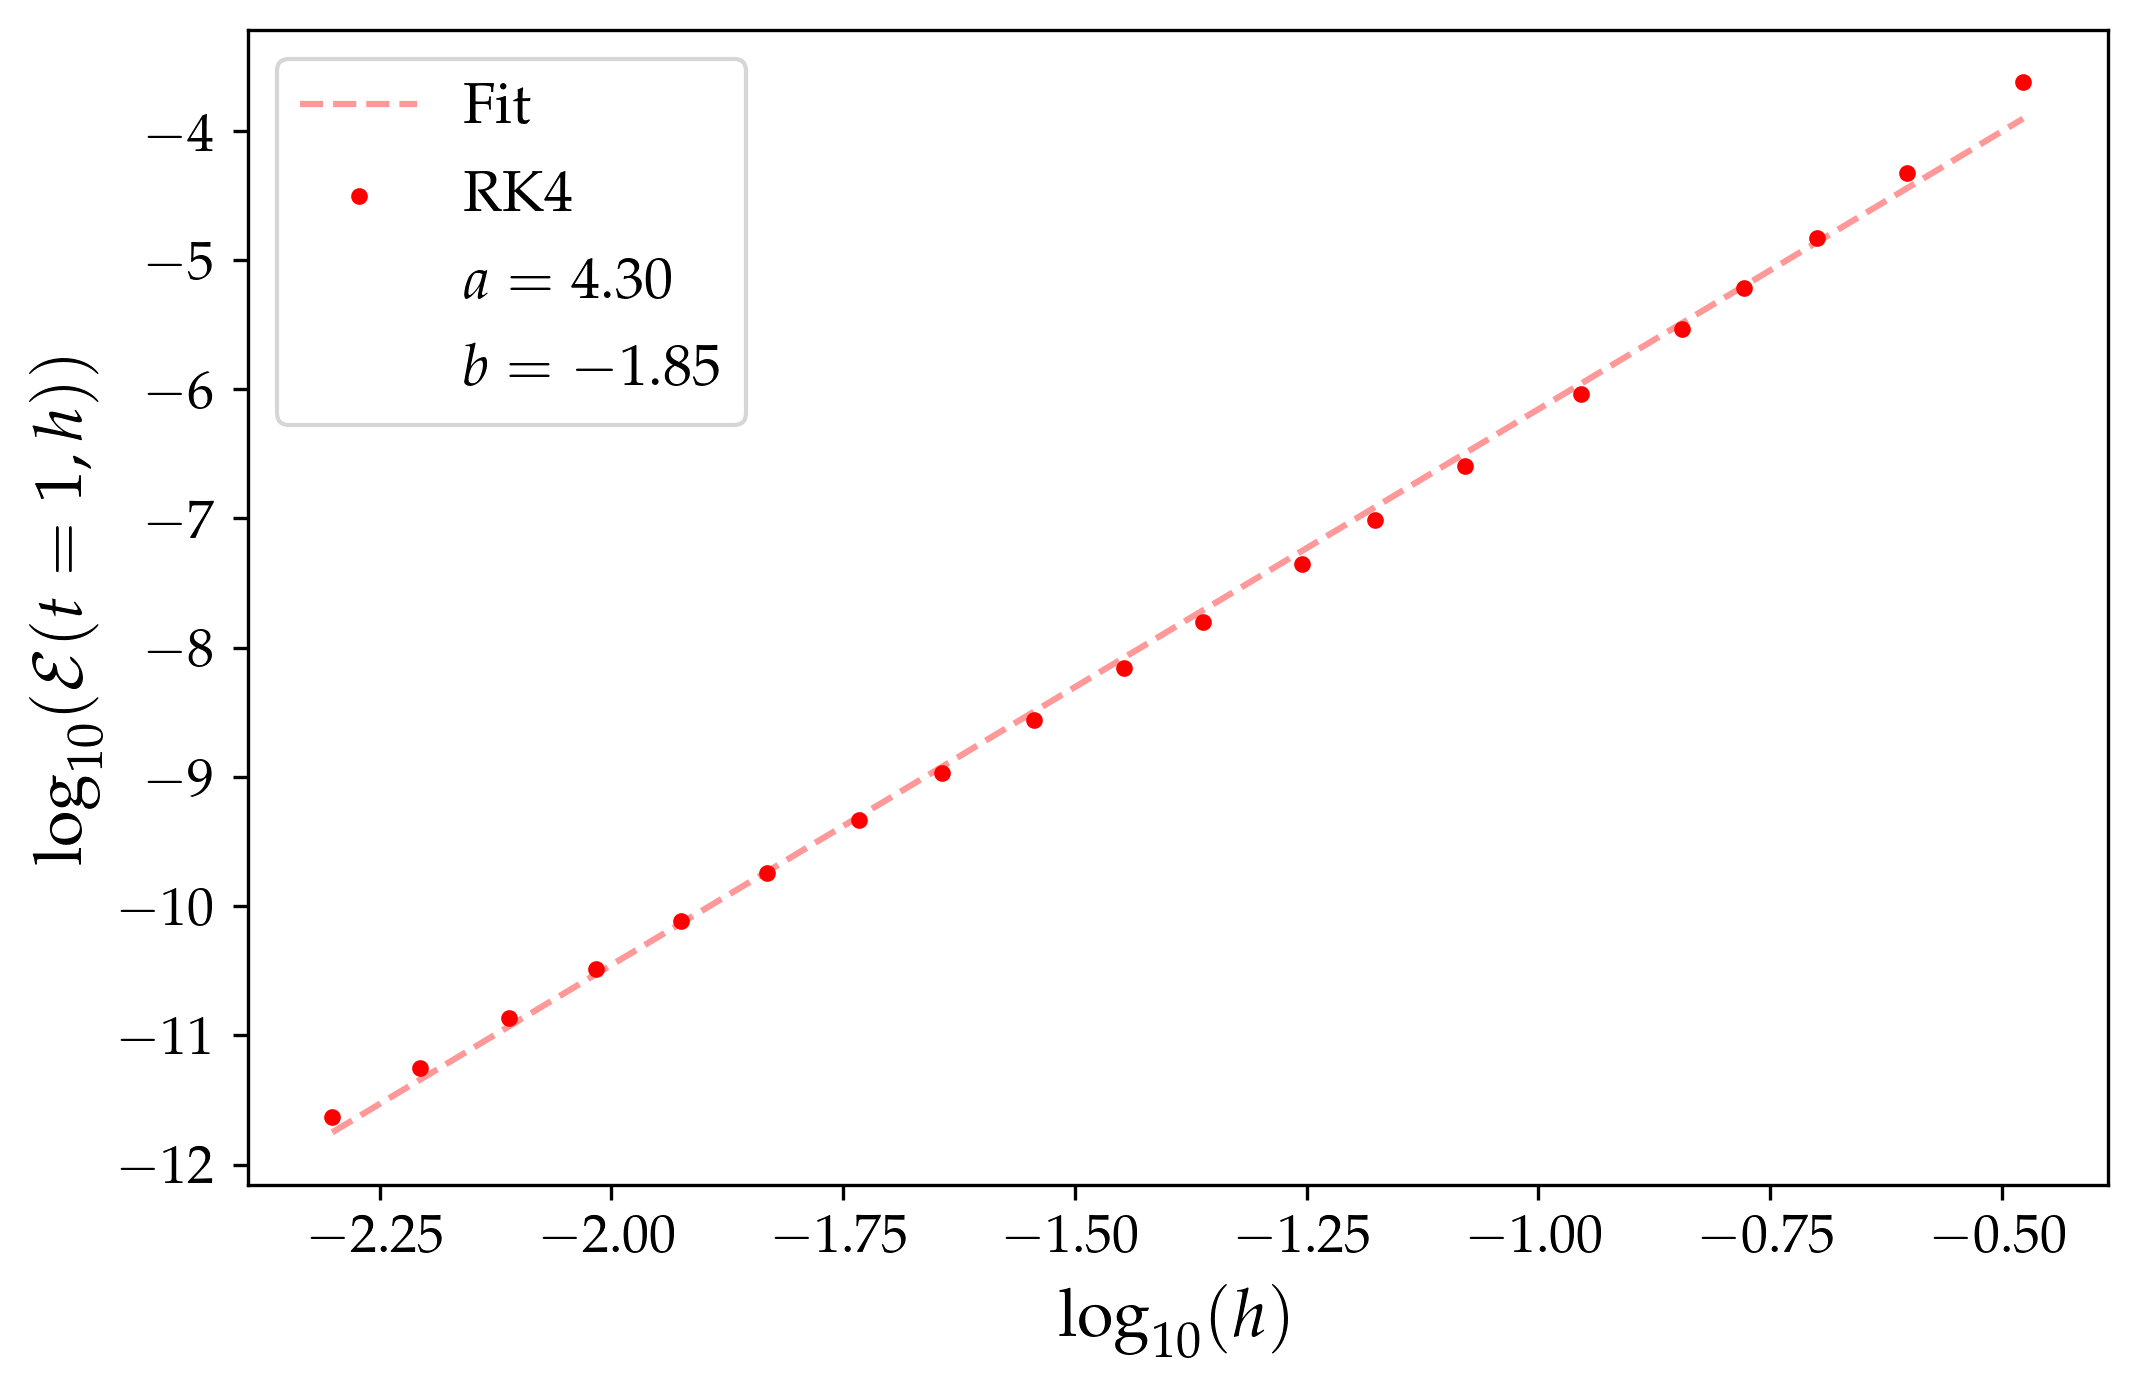
\includegraphics[width=0.8\linewidth]{images/17/17 - 2/fit_rk4.png}
    \caption{Fit del metodo RK4: si verifica la convergenza quartica.}
    \label{fig: fit_rk4}
\end{figure}

\newpage









% \section{Esercizio XXX}
% \subsection{Problem Statement}
% \subsection{Premessa Teorica}
% \subsection{Metodi Numerici e Algoritmi}
% \subsection{Risultati e Discussione}
% \newpage


